\documentclass[11pt,a4paper,oneside]{book}
\usepackage{a4wide}                     % Iets meer tekst op een bladzijde
\usepackage[dutch,english]{babel}       % Voor nederlandstalige hyphenatie (woordsplitsing)
\usepackage{amsmath}                    % Uitgebreide wiskundige mogelijkheden
\usepackage{amssymb}                    % Voor speciale symbolen zoals de verzameling Z, R...
\usepackage{url}                        % Om url's te verwerken
\usepackage{graphicx}                   % Om figuren te kunnen verwerken
\usepackage{xspace}                     % Magische spaties na een commando
\usepackage[latin1]{inputenc}           % Om niet ascii karakters rechtstreeks te kunnen typen
\usepackage{float}                      % Om nieuwe float environments aan te maken. Ook optie H!
\usepackage{flafter}                    % Opdat floats niet zouden voorsteken
\usepackage{listings}                   % Voor het weergeven van letterlijke text en codelistings
\usepackage{marvosym}                   % Om het euro symbool te krijgen
\usepackage{textcomp}                   % Voor onder andere graden celsius
\usepackage{fancyhdr}                   % Voor fancy headers en footers.
\usepackage{graphics}			% Om figuren te verwerken.
\usepackage[nottoc]{tocbibind} % Bibliografie in ToC; zie tocbibind.dvi
\usepackage{longtable}
\usepackage{pdfpages}  % pdf pagina's importeren
\usepackage{subcaption}
\usepackage{setspace}

\newcommand{\npar}{\par \vspace{2.3ex plus 0.3ex minus 0.3ex} \noindent}	% Om witruimte te krijgen tussen paragrafen
\graphicspath{{figuren/}}               % De plaats waar latex zijn figuren gaat halen.
\usepackage[font=small,labelfont=bf,skip=1pt]{caption}

\usepackage[a4paper,plainpages=false]{hyperref}    % Om hyperlinks te hebben in het pdfdocument.
\newcommand{\command}[1]{\lstinline[basicstyle=\tt]{#1}\xspace} %Voor commando's
\hyphenation{con-vo-lu-tio-neel}

% Het bibliografisch opmaak bestand.
\bibliographystyle{enapalike}

\renewcommand{\chaptermark}[1]{\markright{\MakeUppercase{#1}}}
\renewcommand{\sectionmark}[1]{\markright{\thesection~#1}}

\newcommand{\headerfmt}[1]{\textsl{\textsf{#1}}}
\newcommand{\headerfmtpage}[1]{\textsf{#1}}

\fancyhf{}
\fancyhead[LE,RO]{\headerfmtpage{\thepage}}
\fancyhead[LO]{\headerfmt{\rightmark}}
\fancyhead[RE]{\headerfmt{\leftmark}}
\renewcommand{\headrulewidth}{0.5pt}
\renewcommand{\footrulewidth}{0pt}

\fancypagestyle{plain}{ % eerste bladzijde van een hoofdstuk
  \fancyhf{}
  \fancyhead[LE,RO]{\headerfmtpage{\thepage}}
  \fancyhead[LO]{\headerfmt{\rightmark}}
  \fancyhead[RE]{\headerfmt{\leftmark}}
  \renewcommand{\headrulewidth}{0.5pt}
  \renewcommand{\footrulewidth}{0pt}
}

\renewcommand{\lstlistoflistings}{\begingroup
   \tocfile{\lstlistlistingname}{lol}
\endgroup}


% anderhalve interlinie (opm: titelblad gaat uit van 1.5)
\renewcommand{\baselinestretch}{1.5}


\hypersetup{
    pdfauthor = {Jasper Vaneessen},
    pdftitle = {One-shot learning van gebaren in een convolutioneel neuraal netwerk},
    pdfsubject = {Scriptie voorgelegd tot het behalen van de academische graad van Master of Science in de 
    industri�le wetenschappen: informatica, juni 2017}
}

\begin{document}
\selectlanguage{dutch}

\frontmatter


% lege pagina (!!)
%\newpage
%\vfil\null
%\newpage

% titelblad (!!)
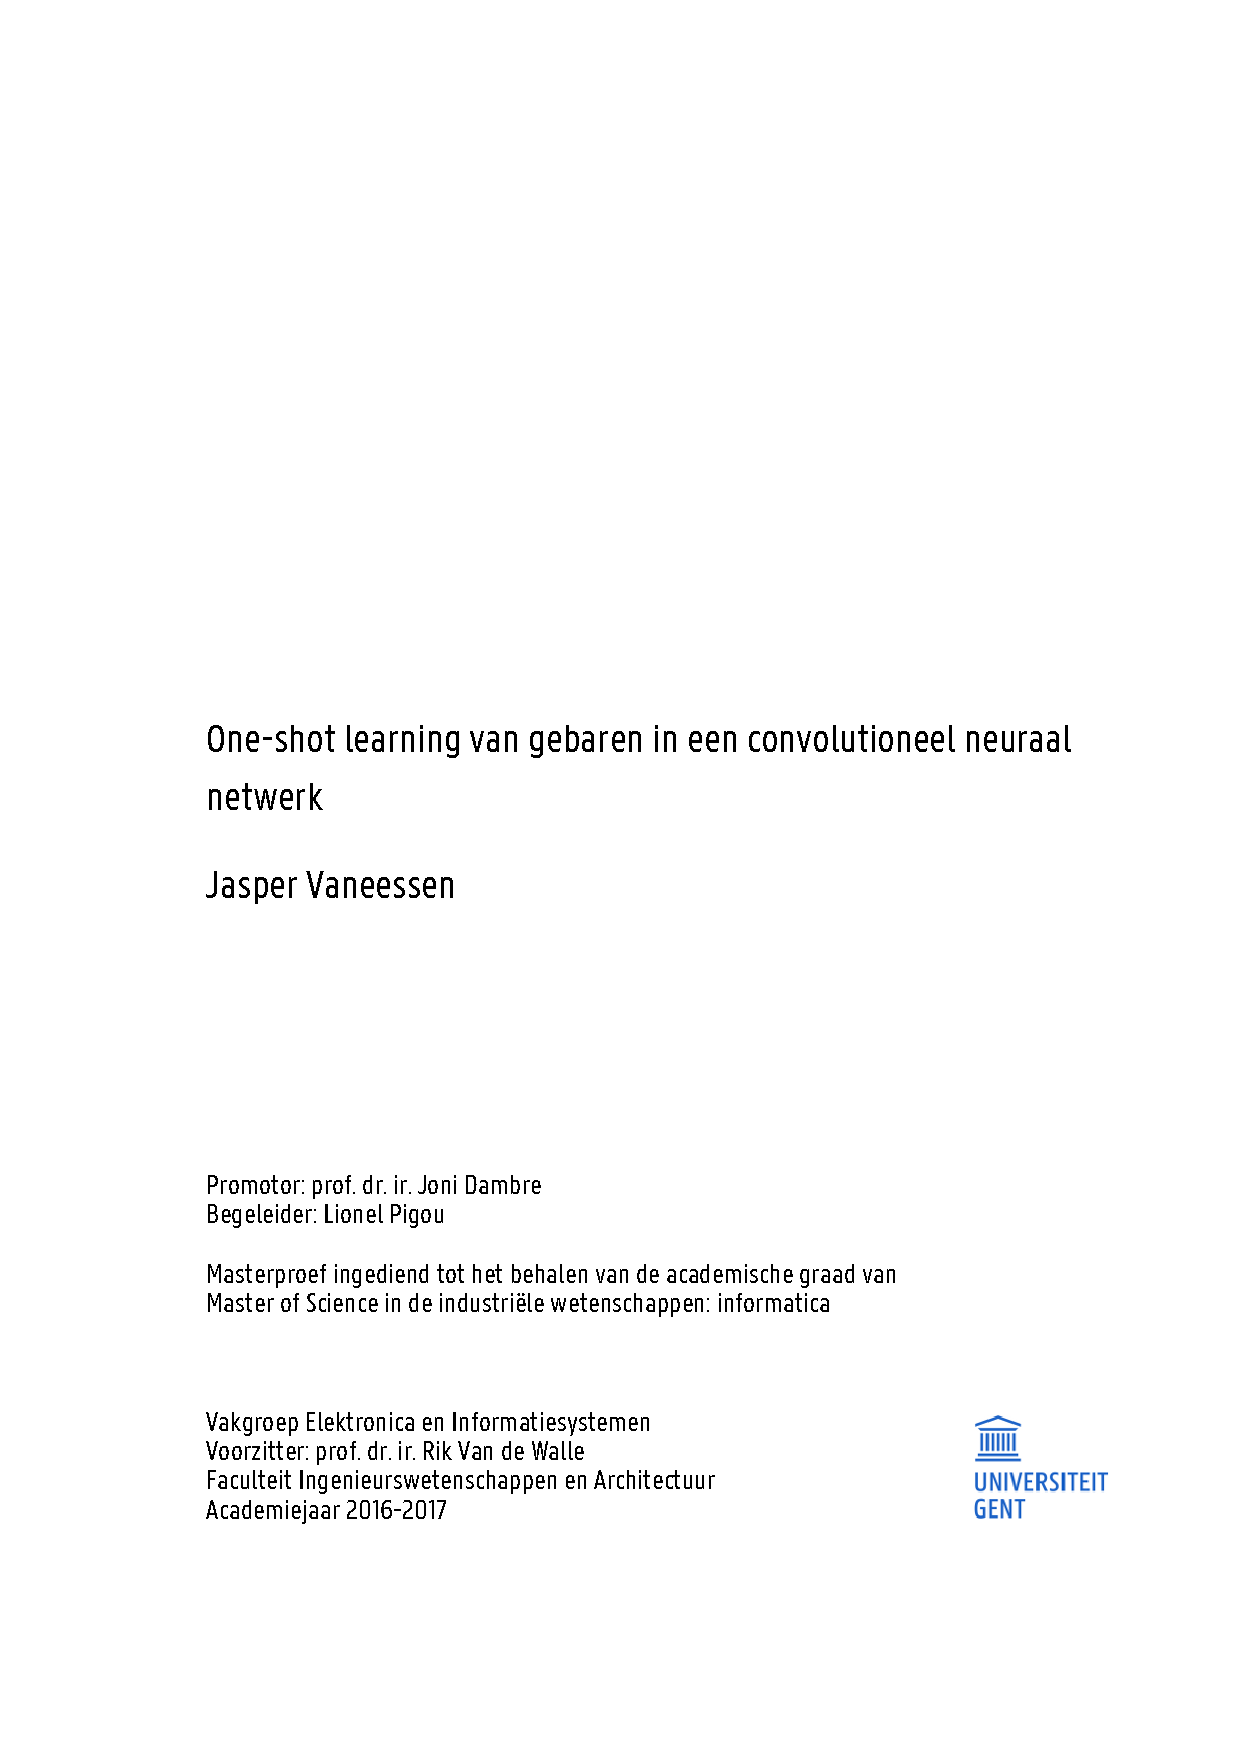
\includepdf[pages={-}]{titelblad}

% geen paginanummering tot we aan de inhoudsopgave komen
\pagestyle{empty}

% voorwoord met dankwoord en toelating tot bruikleen (ondertekend)

\chapter*{Toelating tot bruikleen}

\vspace{1.5cm}

\noindent
``De auteur geeft de toelating deze scriptie voor consultatie beschikbaar
te stellen en delen van de scriptie te kopi\"eren voor persoonlijk
gebruik.\\
Elk ander gebruik valt onder de beperkingen van het auteursrecht,
in het bijzonder met betrekking tot de verplichting de bron uitdrukkelijk
te vermelden bij het aanhalen van resultaten uit deze scriptie.''

\addvspace{4cm}

\noindent Jasper Vaneessen, juni 2017

\chapter{Voorwoord}

\begin{slshape}
\renewcommand{\baselinestretch}{1.2}
\small\normalsize

Vele mensen hebben meegeholpen aan de totstandkoming van deze masterproef. Ik wil graag van de gelegenheid gebruik maken om hen te bedanken.

\npar Eerst en vooral zou ik graag mijn promotor, prof. dr. ir. Joni Dambre, willen bedanken voor haar uitstekende begeleiding tijdens het opstellen van dit werk. Haar inzicht en kritische vragen hebben een duidelijke meerwaarde met zich meegebracht.

\npar Ook wil ik graag mijn begeleider, Lionel Pigou, bedanken voor het delen van zijn expertise, zijn passie en interesse voor machine learning en voor alle raad tijdens afgesproken en onafgesproken momenten. 

\npar Vervolgens wil ik graag een woord van dank richten tot mevrouw Leen Brouns, bij wie ik terecht kon met vragen en zorgen doorheen mijn opleiding.

\npar Voor het nalezen van deze scriptie wil ik graag Joke Van Eessen, Lionel Pigou, Tomas Dupont en Jan Delaeter bedanken.

\npar Graag bedank ik ook mijn ouders en zus, voor hun geduld, steun en vertrouwen tijdens het vervolmaken van mijn opleiding. 

\npar Ten slotte bedank ik graag in het bijzonder mijn vriendin, Joke. Voor haar eeuwige geduld, haar geruststellende woorden en haar luisterend oor waar ik altijd op kan rekenen.


\addvspace{4cm}

\noindent Jasper Vaneessen, juni 2017
\end{slshape}



% overzicht
%  Overzichtsbladzijde met samenvatting

\newpage
\addcontentsline{toc}{chapter}{Overzicht}
{
\setlength{\baselineskip}{12pt}
\setlength{\parindent}{0pt}
\setlength{\parskip}{6pt}

\chapter{Overzicht}
\begin{center}

\vspace{5mm}
\renewcommand{\baselinestretch}{1.1}
\noindent \textbf{
One-shot learning van gebaren in een convolutioneel neuraal netwerk
} \\
\renewcommand{\baselinestretch}{1.3}
\normalsize
Jasper Vaneessen
\vspace{5mm}
\end{center}

Promotor: Prof.~Dr.~Ir.~Joni~\textsc{Dambre}\\
Begeleider: Ir.~Lionel~\textsc{Pigou}

\vspace{5mm}

Masterproef ingediend tot het behalen van de academische graad van\\
\textsc{Master of Science in de industri\"ele wetenschappen:\\ informatica}

\vspace{5mm}

Vakgroep Elektronica en Informatiesystemen\\
Voorzitter: Prof.~Dr.~Ir.~Rik~\textsc{Van de Walle}

\vspace{5mm}

Faculteit Ingenieurswetenschappen \& Architectuur\\
Academiejaar 2016-2017
Universiteit Gent





\section*{Trefwoorden}
gebarenherkenning, convolutionele neurale netwerken, machine learning, deep learning, one-shot learning
}

\newpage % strikt noodzakelijk om een header op deze blz. te vermijden


% abstract
%\addcontentsline{toc}{chapter}{Extended abstract}
%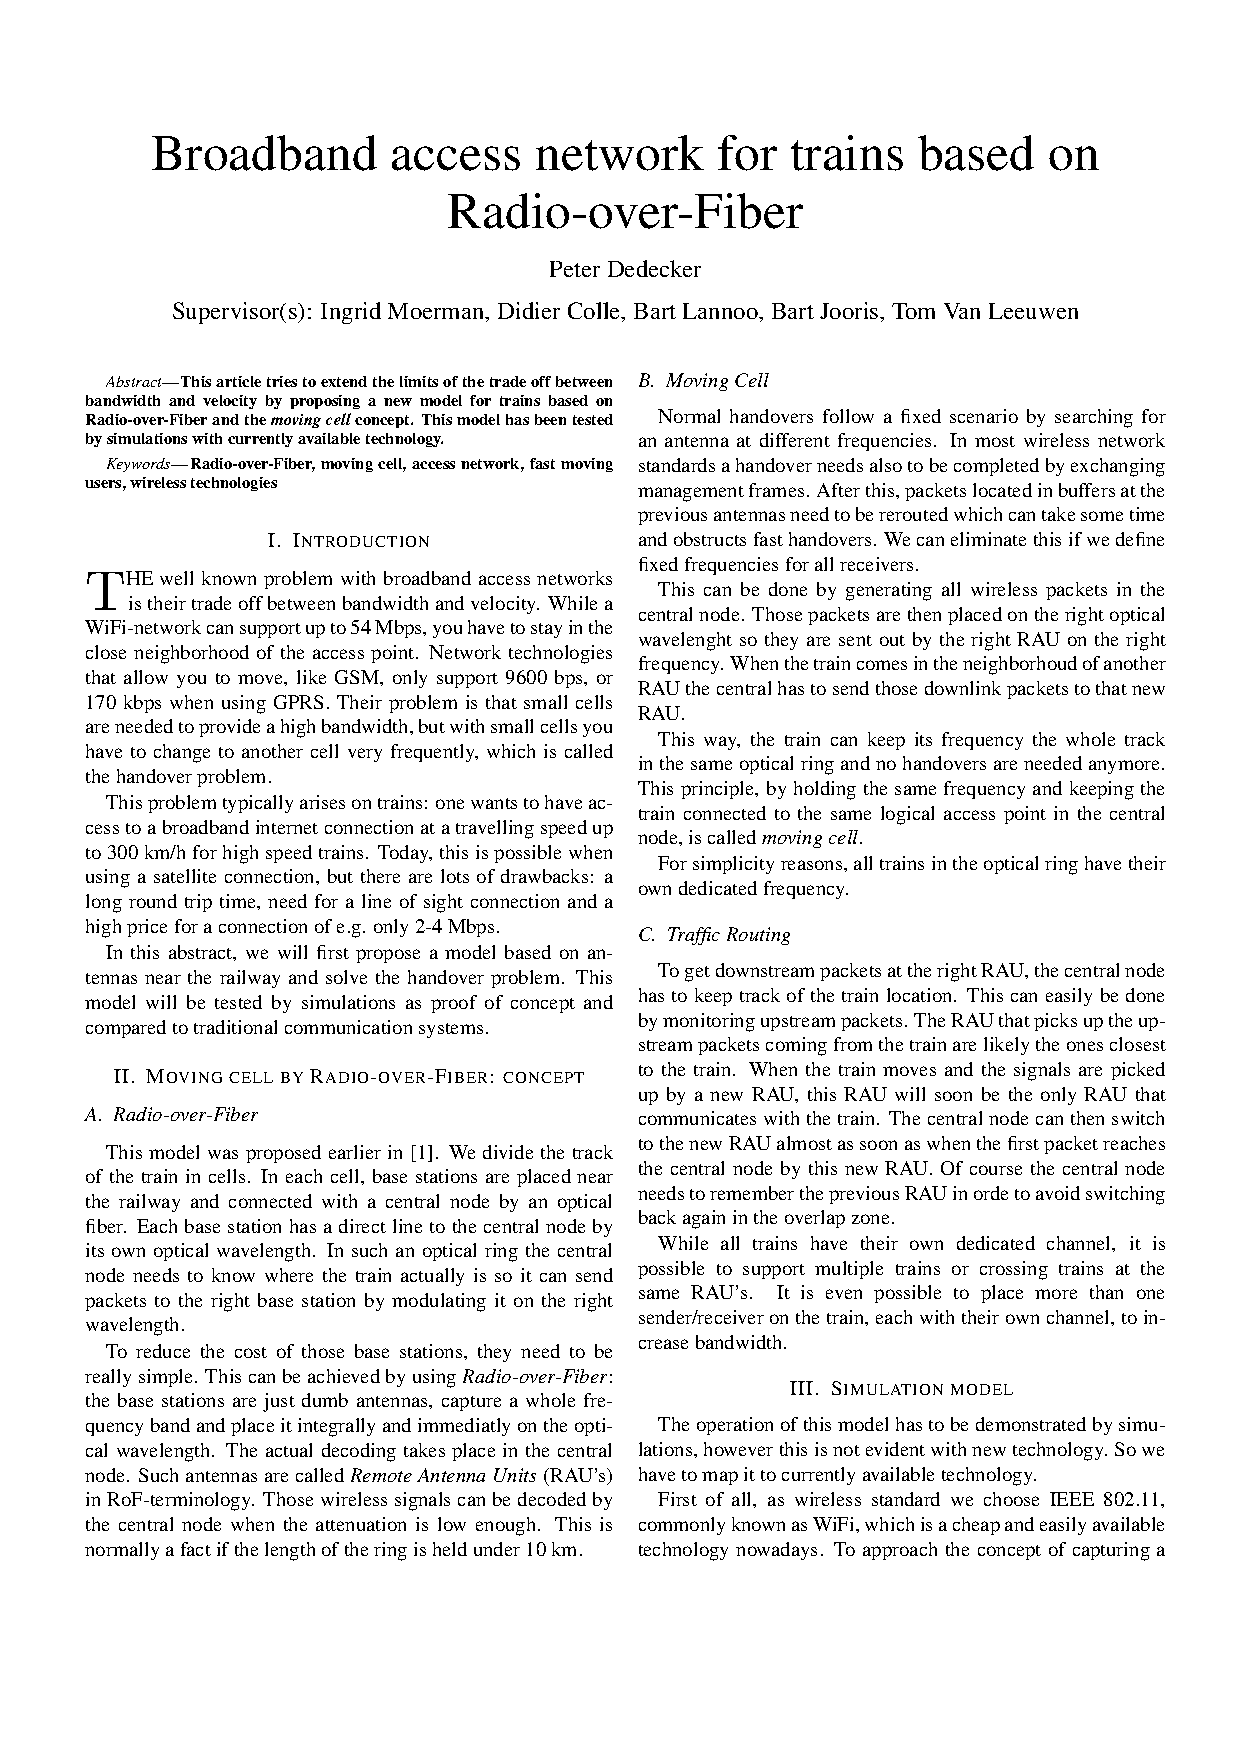
\includepdf[pages=-]{../abstract/abstract.pdf}

\pagestyle{fancy}
\renewcommand{\baselinestretch}{1.08} 	% De interlinie afstand wat verkleinen.
\small\normalsize                       % Nodig om de baselinestretch goed te krijgen.
%\addcontentsline{toc}{chapter}{Inhoudsopgave}
\tableofcontents
\renewcommand{\baselinestretch}{1.2} 	% De interlinie afstand wat vergroten.
\small\normalsize                       % Nodig om de baselinestretch goed te krijgen.
\chapter{Afkortingen}

\renewcommand{\baselinestretch}{1.5}
\small\normalsize
\begin{longtable}{ll}
	ANN & Artifici\"eel Neuraal Netwerk \\
	CNN & Convolutioneel Neuraal Netwerk \\
\end{longtable}


\mainmatter
\chapter{Inleiding}
\section{Gebarentaal}

Gebarentaal is in de eerste plaats een taal. Taal is een begrip dat moeilijk te defini\"eren valt en de meeste pogingen hiertoe beperken zich tot gesproken taal. Een definitie die ook voor gebarentaal kan gebruikt worden is: een natuurlijk ontstaan communicatiemidddel waarmee je kan communiceren over alles wat je denkt, ziet, voelt en droomt. \cite{bron}

\npar Gesproken taal en gebarentaal verschillen in de manier waarop gecommuniceerd wordt: oraal-auditief tegenover gestueel-visueel. Door middel van hand-, hoofd- en armbewegigingen wordt een woord ``uitgesproken'' en vervolgens visueel waargenomen.

\npar Een gebarentaal onstaat, net zoals een gesproken taal, spontaan en natuurlijk door contact tussen mensen. Net door deze spontane ontwikkeling is er geen universele gebarentaal. Evenals we verschillende gesproken talen en dialecten kennen per land of regio zijn er ook verschillende gebarentalen \cite{VGT-standard}. In Nederland is er bijvoorbeeld de Nederlandse Gebarentaal (NGT) en in Belgi\"e de Vlaamse Gebarentaal (VGT) en de Waalse Gebarentaal (la Langue des Signes de Belgique Francophone, LSFB). VGT verschilt dan weer van provincie tot provincie, met de grootste verschillen tussen West-Vlaanderen en Limburg, de twee verst uiteenliggende regio's.

\npar Een gebarentaal heeft een eigen grammatica en lexicon. Het lexicon of de gebarenschat is de verzameling van alle woorden of gebaren in de taal. Het lokale gebarenschat moet volledig onafhankelijk van het lokale woordenschat worden beschouwd.
\\Bepaalde woorden uit de ene taal kunnen niet eenduidig vertaald worden in een andere taal. Het woord "gezelligheid" kent bijvoorbeeld geen Engelse vertaling en voor het Duitse "fingerspitzengef\"uhl" hebben we in de Nederlandse taal ook geen alternatief.
\\Tussen een gebarentaal en een gesproken taal geldt dezelfde verhouding. Er is niet altijd een een-op-een relatie tussen een woord en een gebaar.

\npar Communicatie tussen doven en horenden is vaak een struikelblok. Sommige doven kunnen liplezen en zo opmaken wat een spreker wil vertellen. Voorwaarde hierbij is dat de spreker goed moet articuleren en natuurlijk niet te snel spreekt.
\\ Er kan ook altijd schriftelijk gecommunciceerd worden maar dit is een erg trage en onpersoonlijke vorm van communicatie. Ook is de bedrevenheid van een dove persoon in het schrijven van een gesproken taal vaak lager dan die van een horende.
\\ Doven kunnen zich ook beroepen op een tolk. Dit kan een vriend zijn die horende is en gebarentaal kent of een beroepstolk. In Vlaanderen kunnen doven terecht bij het Vlaams Communicatie Assistentie Bureau voor Doven (CAB) om een tolk in te huren. De Vlaamse overheid betaalt een aantal tolkuren terug. Onder andere achttien tolkuren voor priv\'edoeleinden, achttien voor sollicitaties en een situatie-afhankelijk aantal tolkuren voor arbeid en beroepsopleiding.
 
\section{Automatische gebarentaalherkenning}
Er is een communicatieprobleem tussen doven en horenden omdat ze niet dezelfde taal spreken. Er zijn ook vele verschillende gebarentalen en dialecten waardoor er tussen doven onderling ook niet altijd vlot gecommuniceerd wordt.
Door het gebruik van hedendaagse technologie moet het mogelijk zijn hierin te helpen en een automatisch herkenningssysteem uit te werken waarmee gebaren in real-time kunnen vertaald worden.

\npar Het herkennen van objecten of gebaren is iets waar de mens niet bij stilstaat. Een pasgeboren kind begint vanaf het openen van de ogen zijn waarneming en herkenningsvermogen te trainen. Terwijl we leren organiseren we vormen, objecten en categori\"en in nuttige taxonomi\"en en linken deze dan later naar onze taal \cite{oneshot-object-cat}. Eenmaal de leeftijd van zes jaar bereikt is kan een kind bijvoorbeeld 104 objectcategori\"en onderscheiden zonder hierbij stil te staan.

\npar Als mens kunnen we gebaren makkelijk differenti\"eren door registratie van armbewegingen, mimiek, houding van de handen en de manier waarop vingers gestrekt of geplooid worden. De neurologische fenomenen die deze vaardigheden kunnen verklaren worden nog steeds onderzocht. 

\npar Een machine of computer kan zien via het gebruik van een camera. Een beeld wordt voorgesteld door een matrix met pixelwaarden die de lichtintensiteit op dat bepaalde punt weergeeft. Traditioneel zijn er grijswaarden- en kleurbeelden maar tegenwoordig wordt ook vaak gebruikt gemaakt van 3D-cameratechnologi\"en, zoals de Microsoft Kinect \cite{kuhn2011kinect}, zodat er een aanvullend dieptebeeld is. Deze beelden gelden dan als de visuele data voor het systeem, daarna moeten specifieke technologiën worden ingezet om nuttige informatie uit deze data te halen.

\npar Een automatisch herkenningssysteem zal moeten leren omgaan met de grote variabiliteit van de invoer. De gebaren die het moet herkennen zullen uitgevoerd worden door mensen van verschillende groottes. De vlotheid van het gebaren tussen ervaren en beginnende gebarentaligen zal ook sterk verschillen. De persoon zal ook niet altijd mooi recht in het midden van het beeld staan of even ver van de camera. Ook links- en rechtshandigheid heeft een invloed op het gebaren evenals de expressiviteit van de spreker.
\\ De aanwezigheid van andere mensen of veel beweging in de achtergrond bemoeilijkt ook het herkennen van gebaren. Daarboven moet ook nog rekening gehouden worden met de lokale belichting, de spreker kan onderbelicht of overbelicht zijn waardoor bepaalde contouren moeilijker te detecteren vallen.

\npar Een compleet gebarentaalherkenningssysteem zal moeten voorzien in gebarensegmentatie, gebarenherkenning en grammaticale samenstelling van gebaren.

\subsection{Gebarensegmentatie}
\npar Wanneer we een persoon die gebarentaal spreekt registreren met een camera krijgen we een continue stroom aan informatie. In een bepaalde tijdspanne kan een persoon een of meerdere gebaren uitvoeren en het is onbekend waneer een gebaar begint of eindigt. De segmentatie van deze gebaren is dus een eerste uitdaging voor een herkenningssysteem. Er is minder belangstelling naar deze ``continue'' gebaarherkenningssystemen omdat vaak wordt uitgegaan van vooraf gesegmenteerde beelden \cite{hmdb-manual-segm}.
\\ Tussen elk gebaar zit er een beweging die de overgang vormt tussen twee gebaren: de bewegingsepenthesis. Armen en handen gaan van eindpositie van het eerste gebaar naar beginpositie van het volgende. \cite{movement-epenthesis} Deze beweging moet gedetecteerd en gefilterd worden willen we een foutloze segmentatie krijgen.

\subsection{Gebarenherkenning}
Eenmaal we weten wanneer een gebaar begint en eindigt kunnen we het gaan identificeren. Uit de verzamelde visuele data wordt nuttige informatie ge\"extraheerd waarmee het model kan beslissen over welk gebaar het gaat. Het beeld wordt omgezet in een beeldrepresentatie, bestaande uit een of meerdere featurevectoren. Deze representatie wordt vervolgens gebruikt door een classificatie methode die het een klasselable geeft.

\npar \cite{gesture-FNN-HMM} stelt een gebaarherkenningssyteem voor die zich focust op de handen. Uit het dieptebeeld van een Kinectcamera wordt de hand gesegmenteerd via thresholding. Drie features worden vervolgens bijgehouden en gebruikt: de verandering van de handvorm, de beweging van de hand in het tweedimensionaal vlak en de beweging van de hand in de diepte (z-as).
\\Er wordt gebruik gemaakt van twee classificatie methodes: Hidden Markov Modellen (HMM) en Fuzzy Neurale Netwerken (FNN). HMM is een classificatietechniek die rekening houdt met het tijdsaspect. FNN is een combinatie van fuzzy (vage) theorie en artifici\"ele neurale netwerken.

\subsection{Grammaticale samenstelling}

%Camera
%Features
%
%Gebaarsegmentatie
%Waar begint een gebaar en waar eindigt het
%Gebaarherkenning
%Welk gebaar en wat betekent het
%Boodschap ontleden --> gebaren samenstellen, grammatica, (bv. letterwoorden, kleur)

\section{One-shot learning}

\subsection{Uitbreidbaarheid herkenningssysteem}
Een taal is voortdurend in verandering.
Het lexicon van een gebarentaal groeit mee met de tijd. Gloednieuwe termen of zaken die voordien geen beschrijving kenden in een gebarentaal worden toegevoegd. Hogescholen en universiteiten gebruikten lange tijd geen gebarentaal waardoor er weinig wetenschappelijke termen opgenomen zijn in de gebarenschat. Gelukkig komen er vandaag steeds meer wetenschappelijke gebaren bij.

\npar Een automatische herkenningssysteem zal moeten leren omgaan met dit groeiende lexicon. Een strategie kan zijn om na verloop van tijd (vanaf een bepaald aantal nieuwe gebaren) het systeem te hertrainen met voorbeelden van de oude gebaren en de nieuwe gebaren. Hierbij wordt er dus vanaf nul gestart en een nieuw model opgebouwd.

\npar Een eerste probleem is het verzamelen van de data. Deep learning methodieken hebben een complexe structuur en erg veel parameters. Om een grote hoeveelheid parameters te optimaliseren voor een taak heb je een grote hoeveelheid data nodig om uit te leren. Als we dus een nieuw gebaar willen bijleren aan een herkenningssysteem hebben we vele voorbeelden nodig van dit ene gebaar, liefst tegen verschillende achtergronden, uitgevoerd door verschillende personen en in verschillende lichtomstandigheden.
\\ Het maken van dergelijke datasets is een erg kostelijke en tijdrovende opdracht.

\npar Het model vanaf nul terug hertrainen vraagt veel tijd en rekenvermogen. Alle vooraf opgedane kennis wordt gewist dus alle tijd en moeite die eerder ge\"investeerd werd is voor niets. Het systeem zal ook minstens evenveel rekentijd nodig hebben als tijdens de opbouw van het vorige model.

\npar Als we zo een aantal keer het herkenningssysteem willen uitbreiden zullen we veel kostbare tijd en energie verspillen.

\subsection{Bijleren bij mensen}





\subsection{One-shot learning in de literatuur}


\npar \cite{oneshot-vis-concepts} stelt een generatief model voor voor het herkennen van handgeschreven karakters. Het vertrekt vanuit de notie dat de mens een teken schrijft in verschillende halen of lijnen en ook zo een nieuw teken leert herkennen. Er wordt een dataset opgebouwd van 1600 tekens die door verschillende gebruikers online geregistreerd worden. Elke lijn die een gebruiker plaatst wordt opgeslaan alsook de volgorde van tekenen. Zo bestaat elk teken uit een opeenvolging van lijnen met verschillende vorm en lengte. De verzameling van al deze lijnen wordt gebruikt als voorafgaande kennis om nieuwe tekens bij te leren met een voorbeeld. Het nieuwe teken wordt door het systeem opgedeeld in lijncomponenten die dan afgetoetst worden tegen het model. Zo ontstaat een nieuwe representatie voor het bijgeleerde gebaar die kan gebruikt worden voor herkenning. Er wordt een nauwkeurigheid van 54.9 \% behaald tegenover 39.6 \% voor een implementatie aan de hand van Deep Boltzman Machines (DBM). Wanneer bij het aanleren van het nieuwe gebaar de lijninformatie van de dataset wordt gebruikt in plaats van die van het systeem zelf wordt een nauwkeurigheid van 63.7 \% waargenomen.

\npar \cite{oneshot-gesture-rgbd} buigt zich over de ChaLearn One-shot Learning Gesture Challenge 2011 en leert vanuit slechts een voorbeeld een gebaar te herkennen zonder enige voorgaande kennis. Er wordt ge\"experimenteerd met een aantal feature descriptors en classificatie methodes waaruit Extended Motion History Images (Extended MHI) en Maximum Correlation Co\"effici\"ent (MCC) als best presterende worden gevonden. Extended MHI  bestaat zelf uit drie representaties: MHI en Inversed recording (INV) focussen zich op bewegingsinformatie respectievelijk in het begin en op het einde van het gebaar terwijl Gait Energy Information (GEI) repetitieve beweging registreert. Het systeem behaalt een Levensteihnafstand van 0.29685 (tussen O en 1 waarbij 0 optimaal) op de validatieset en presteert zeer goed op gebaren waarin er veel beweging is. De twee meer statische gebaren uit de dataset worden het minst goed gededecteerd met een nauwkeurigheid lager dan 45 \%.

\npar \cite{oneshot-video-segm} stelt een CNN voor die uit een voorbeeld de voorgrond van de achtergrond onderscheidt in een video. Het CNN wordt vooraf getraind op de ImageNet dataset. Een dataset van 1,2 miljoen afbeeldingen uit meer dan duizend categori\"en. Door deze pre-training op een zeer ruime dataset is het model algemeen en leert het eigenlijk wat 'een object' is. Hierna wordt het model verfijnd voor het volgen van een voorgrondsobject uit een video. Het eerste frame van de video wordt gemaskeerd en hierop stelt het model zich af. Deze architectuur verbetert de state-of-the-art op de Densely Annotated Video Segmentation (DAVIS) dataset met 11.2 \% (79.8\% vs 68.0\%).

\section{Doelstelling}









 
\chapter{Technische aspecten}
\section{Machine Learning}
\subsection{Inleiding}
\npar Leren is een veelzijdig fenomeen dat bestaat uit  verschillende processen: het verkrijgen van declaratieve kennis, het ontwikkelen van motorische en cognitieve vaardigheden door instructie en ervaring, het organiseren van nieuwe kennis in algemene representaties en het ontdekken van nieuwe feiten via observatie en experimentatie.
\npar Sinds het begin van het computertijdperk proberen onderzoekers het menselijk leren na te bootsen en deze processen te vertalen naar de informatietheorie. Het machinaal leren is nog steeds een erg uitdagend doel in de kunstmatige intelligentie (KI).

\npar Deze vorm van KI is dus volledig data gedreven tegenover traditionele methoden die zich beroepen op handgemaakte regels. Het computerprogramma wordt niet expliciet geprogrammeerd om een taak uit te voeren maar vertrekt vanuit een algemeen model. Het model leert eerst uit voorbeelden en kan daarna voorspellingen maken op nieuwe invoer.

\npar We kunnen zeggen dat een computerprogramma of machine leert als het zijn performantie op een bepaalde taak verbetert met ervaring \cite{machine_overview}.  Het leren gebeurt door de optimalisatie van de parameters van het predictief model door middel van een algoritme uit de machine learning. Het model wordt een aantal voorbeelden gegeven om uit te leren: de trainset. De uitvoer van het model wordt ge\"evalueerd aan de hand van een prestatiemaat. Deze prestatiemaat vertelt hoe correct de voorspelling is en bepaalt de mate waarin het model verder gecorrigeerd dient te worden.

\npar Machine learning algoritmes kunnen opgedeeld worden in drie categori\"en op basis van leerstijl: gesuperviseerd, ongesuperviseerd en semi-gesuperviseerd leren. De supervisie slaat op het gebruik van de correcte uitgangswaarde tijdens het trainen.

\npar Een ongesuperviseerde leerstijl vertrekt uit een dataset zonder klasselabels of correcte voorspellingswaarde. Er wordt een model opgebouwd dat bepaalde structuren deduceert. Dit kan zijn om algemene regels te extraheren, om redundantie te verminderen of om gegevens te groeperen volgens gelijkenis (clustering).

\npar Bij gesuperviseerde methodes wordt een trainset gebruikt die zowel de invoervector als de te voorspellen waarde bevat. Problemen die vaak via gesuperviseerd leren worden aangepakt zijn classificatie en regressie. Classificatie tracht ingevoerde voorbeelden in te delen in discrete categori\"en om bijvoorbeeld objecten te herkennen zoals in \cite{cnn-krizhevsky}. Bij regressie is de uitvoer van het model een continue variabele zoals bijvoorbeeld de prijs van een appartement gegeven zijn oppervlakte.

\npar Semi-gesuperviseerde methodes zijn e+9en mengvorm van de voorgaande twee. De dataset is een mengeling van gelabelde en ongelabelde voorbeelden. Hierbij is er een gewenste indeling, weergegeven door de gelabelde data, maar het model moet zelf de indeling zien te maken.


\subsection{Gesuperviseerde classificatie}

\npar De machine learning in dit onderzoek valt onder de gesuperviseerde classificatie. Een classificatieprobleem kan algemeen als volgt worden omschreven:
\npar Gegeven een trainset T:
\begin{equation}
T = \{ ( x^{(n)}, y^{(n)})\},\quad x^{(n)}\in\mathbb{R}^D, y^{(n)}\in\{0,1,...,C\}, n=1,...,N
\end{equation}
met $x^{(n)}$ het n-de datavoorbeeld en $y^{(n)}$ zijn klasselabel. C staat voor het aantal discrete categori\"en of klasses, D het aantal dimensies van de invoervariabelen en N het aantal trainingsvoorbeelden. Nu kunnen we het classificatieprobleem uitdrukken als de benadering van een model $f$ met parameters $\theta$:
\begin{equation}\label{eq:classifier}
f(x,\theta) = y,\quad\forall(x,y) \in T
\end{equation}
zodat we na deze schatting vanuit $f$ en $\theta$ voorspellingen kunnen maken op basis van nieuwe data: $f(x_{nieuw},\theta)=y', \quad y' \in\{0,1,...C\}$

\npar Figuur \ref{fig:alg-class-model} geeft een schematische weergave van de opbouw van een classificatiemodel. Het schatten van $f$ en $\theta$ wordt uitgevoerd door een techniek uit de machine learning en geeft ons het uiteindelijke predictief model $f(x,\theta) = y$. De samples worden meestal verwerkt voor ze als input worden doorgegeven aan het model. In het geval van classificatie van video en afbeeldingen worden er technieken uit de beeldverwerking gebruikt om relevante informatie uit het beeld te halen. Welke specifieke techniek er gebruikt wordt is een keuze die erg bewust moet gemaakt worden en een grote invloed heeft op de performantie van het classificatiemodel. Deze informatie wordt gebundeld in een featurevector $x$ en aan het ML algoritme gegeven. Vanuit de verkregen featurevectoren en de kennis van het correcte klasselabel wordt het predictief model dan geoptimaliseerd.
\npar Eenmaal het model voldoende geleerd heeft kan het predictief model gebruikt worden in een productieomgeving om nieuwe voorbeelden, al dan niet correct, te classificeren.
\npar Het model dat in dit onderzoek gebruikt wordt, is dat van het artificieel neuraal netwerk, een veel gebruikt predictief model voor classificatie. In Sectie \ref{sec:ann} wordt deze techniek dan ook verder besproken.
\begin{figure}[t]
	\centering
	\def\svgscale{0.85}
%	\def\svgwidth{\columnwidth}
	\input{figuren/figuur-classificatieML.pdf_tex}
	\caption{Schematische weergave van het opstellen van een predictief model met behulp van machine learning technieken \label{fig:alg-class-model}}
\end{figure}

\subsection{Overfitting}
Stel dat een student kunstwetenschappen voor zijn examen het werk van verschillende kunstenaars moet herkennen. Hij krijgt een boek met daarin foto's van verschillende schilderijen samen met de naam van de uitvoerder. Indien de student al deze voorbeelden met hun antwoord vanbuiten leert en op het examen net dezelfde schilderijen als in het boek zou voorgeschoteld krijgen, dan zal hij erg hoog scoren. Krijgt hij echter ongeziene werken van dezelfde schilders, dan zal zijn score veel lager liggen. Hij heeft geen onderliggende eigenschappen uit de beelden gehaald die terugkomen in ander werk maar memoriseerde gewoon werk en uitvoerder dus heeft hij veel moeite met het categoriseren van de nieuwe voorbeelden. Dit is een informeel voorbeeld van overfitting.

\npar Bij overfitting beschrijft het predictief model de ruis en fouten in het signaal in plaats van de gewenste onderliggende patronen en kenmerken van de gegeven taak. Het komt voor wanneer het model complex is en vele parameters heeft in vergelijking met het aantal trainingsvoorbeelden. Een model dat ``overfit'' is heeft een laag voorspellend vermogen op ongeziene data. Het model is niet algemeen of gegeneraliseerd en  memoriseert de data. 

\begin{figure}
	\centering
	\def\svgscale{0.7}
	%	\def\svgwidth{\columnwidth}
	\input{figuren/overfitting.pdf_tex}
	\caption{Plot van trainings- en validatiefout ter illustratie van overfitting en de early stopping techniek.}
	\label{fig:overfitting}
\end{figure}

\npar Het risico op overfitten komt voort uit het feit dat de prestatiemaat voor de training van het model niet correct de effectiviteit van het model weergeeft en er daardoor te laat gestopt wordt met trainen. De training van een model gebeurt via optimalisatie van zijn prestatie op een training set. De werkelijke performantie wordt echter gegeven door prestatie op ongeziene data. Net om deze reden wordt de dataset opgesplitst in drie delen: training-, validatie- en testset.
\npar Om een zo goed mogelijk predictief model te maken wordt een evaluatiescore op de validatieset geoptimaliseerd. Deze data is nog onbekend voor het model en geeft dus een betere aanduiding van zijn performantie. Figuur \ref{fig:overfitting} geeft de validatie- en trainingsfout weer tijdens het trainen van een predictief model. Wanneer de trainingsfout blijft dalen maar de validatiefout stagneert of stijgt is er sprake van overfitting. Nu kan er gekozen worden om de training vroegtijdig te stoppen teneinde geen generalisatie te verliezen. Deze techniek wordt \textit{early stopping} genoemd.

\npar Om na afloop een finale evaluatie van het model te maken wordt zijn prestatie op de testset gemeten. Het model heeft de voorbeelden uit deze set nog nooit eerder gezien waardoor de testscore representatief is voor het voorspellingsvermogen van het model. De testset mag nooit gebruikt worden om aanpassingen aan het model te maken, hiervoor dient de validatieset.

\section{Artificieel neuraal netwerk}\label{sec:ann}
\subsection{Inleiding}
\begin{figure}
	\centering
	\begin{subfigure}{.5\textwidth}
		\centering
		\input{figuren/neuron.pdf_tex}
		\caption{Artificieel neuron.}
		\label{fig:neuron}
	\end{subfigure}%
	\begin{subfigure}{.5\textwidth}
		\centering
		\input{figuren/ANN-alg.pdf_tex}
		\caption{Artificieel neuraal netwerk}
		\label{fig:ANN}
	\end{subfigure}
	\caption{Een ANN (\textbf{b}) met een invoerlaag, twee verborgen lagen en een softmax uitvoerlaag samen met zijn bouwsteen, het artificieel neuron (\textbf{a}). Het rood omkaderde gedeelte kan meerdere malen herhaald worden om een dieper en complexer netwerk te maken.}
	\label{fig:test}
\end{figure}
Een lange rekensom uitwerken is iets wat de mens liever overlaat aan een rekenmachine of computer. Alle bits van een rekensom zijn even belangrijk en bepalend voor de uitkomst. Op dit vlak is een computer veel effici\"enter en betrouwbaarder dan ons brein. Onze hersenen zijn veel bedrevener in andere taken zoals het indelen van objecten volgens gelijkenissen of het herkennen van een persoon.
\npar Het is deze gedachte die vele onderzoekers ertoe bracht een artificieel neuraal netwerk (ANN) uit te bouwen. Het menselijke brein is een erg complex neuraal netwerk bestaande uit meer dan 86 miljard neuronen. Dit zijn de bouwstenen van ons zenuwstelsel en ze staan in voor het verwerken en overdragen van informatie. Ze nemen input aan van een of meerdere neuronen, verwerken deze signalen en sturen al dan niet een signaal door naar  andere neuronen. In Figuur \ref{fig:neuron} is een weergave te zien van een artificieel neuron, de bouwsteen van het ANN. De functionaliteit van dit neuron bootst deze van het biologisch neuron na en wordt als volgt gedefini\"eerd:
\begin{equation}\label{eq:neuron}
n = a\bigg(b+\sum_{i=1}^{D}w_ix_i\bigg)
\end{equation}
met $n$ de uitvoer van het neuron, $a$ de \textit{activatiefunctie}, $b$ de bias, $x_i$ de $i$-de invoer en $w_i$ de gewichten van zijn respectievelijke inkomende verbindingen.



\npar Deze artifici\"ele neuronen worden gegroepeerd in lagen om een ANN te vormen zoals afgebeeld in Figuur \ref{fig:ANN}. Alle lagen worden onderling volledig verbonden: elk neuron krijgt invoer van alle neuronen uit de voorgaande laag en geeft zijn uitvoer door aan alle neuronen van de volgende laag. Deze lagen worden dan ook vaak \textit{dense layers} genoemd vanwege hun verbindingsdichtheid. Tussen de neuronen van een laag in zijn er geen verbindingen. 
\npar Hier beschouwen we enkel \textit{feedforward neurale netwerken}. Aan het begin van het netwerk hebben we de invoerlaag met evenveel neuronen, of knopen, als de dimensie van de featurevectoren. De invoer propageert zich van links naar rechts door het netwerk tot het bij de uitvoerlaag komt. Omdat de uitvoer van de binnenste lagen niet meteen zichtbaar is worden deze de verborgen lagen genoemd.
\npar De uitvoer van de verschillende lagen uit het ANN in Figuur \ref{fig:ANN} kunnen we als volgt beschrijven:
\begin{equation}
\begin{aligned}
h^{(1)}_j\quad=&\quad a\bigg(b^{(1)}+\sum_{i=1}^{D}w^{(1)}_{i,j}x_i\bigg),\quad j=1,...,M_1\\
h^{(2)}_j\quad=&\quad a\bigg(b^{(2)}+\sum_{i=1}^{M_1}w^{(2)}_{i,j}h^{(1)}_i\bigg),\quad j=1,...,M_2\\ 
y_j\quad=&\quad a\bigg(b^{(3)}+\sum_{i=1}^{M_2}w^{(3)}_{i,j}h^{(2)}_i\bigg),\quad j=1,...,C 
\end{aligned}
\end{equation}
met $D$ het aantal invoerparameters, $M_1$ het aantal verborgen knopen in de eerste laag, $M_2$ het aantal verborgen knopen in de tweede laag en $C$ het aantal te voorspellen klassen. $M_1$ en $M_2$ zijn parameters van het model die niet trainbaar zijn maar gekozen worden. De ideale instelling van deze zogenaamde \textit{hyperparameters} wordt bekomen na een iteratief proces van hyperparameteroptimalisatie. Ze worden aanvankelijk gekozen vanuit ervaring en vuistregels uit de literatuur. Door de prestatie van het model te evalueren tegenover de validatieset kunnen deze parameters stelselmatig geoptimaliseerd worden. Elk model heeft zo meerdere hyperparameters wiens ideale waarden experimenteel moeten worden ingesteld.
\npar Het is mogelijk en wenselijk om nog meer verborgen lagen toe te voegen. Het omkaderde gedeelte in Figuur \ref{fig:ANN} kan een aantal keer herhaald worden om zo het model toe te laten een complexere structuur te modelleren.
\begin{figure}[ht]
	\begin{center}
		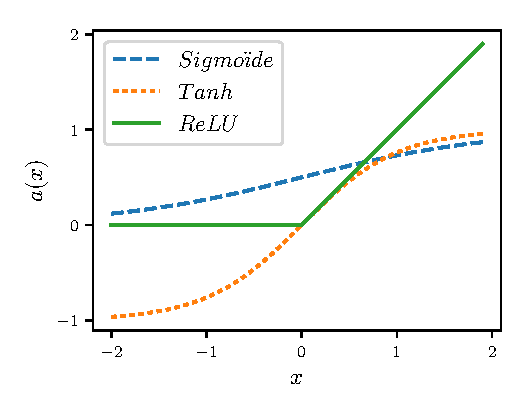
\includegraphics[width=8cm,keepaspectratio]{figuren/activatiefuncties.pdf}
		\caption{Weergave van de drie meest populaire activatiefuncties voor classificatie doeleinden \label{fig:activatie-fun}}
	\end{center}
\end{figure}
\npar De activatiefunctie $a(x)$ uit (\ref{eq:neuron}) is van groot belang in een ANN aangezien ze zorgt voor niet-lineariteit. Moest deze er niet zijn kan elk neuraal netwerk met een verborgen laag vervangen worden door een model zonder, aangezien de samenstelling van lineaire transformaties zelf een lineaire transformatie is. Figuur \ref{fig:activatie-fun} geeft drie van de meeste gebruikte niet lineaire activatiefuncties weer. In dit onderzoek zal gebruik gemaakt worden van de rectifier activatiefunctie:
\begin{equation}
\quad a(x) = max(0,x)
\end{equation}
Een neuron wordt vaak vernoemd naar de activatiefunctie die ze gebruikt. In dit geval spreken we van een Rectified Linear Unit (ReLU). Het gebruik van ReLU's wordt gestaafd in de literatuur omtrent gesuperviseerde \textit{deep learning}: \cite{ReLU}, \cite{lionel} en \cite{wu_deep_2016}. Een ReLU zal alle negatieve waarden afbeelden op 0 en alle positieve op zichzelf.

\npar Aan de uitgang van het ANN worden geen ReLU's geplaatst maar hebben we de softmaxlaag. De uitvoer van de softmaxlaag geeft de voorspelde probabiliteit per klasse weer. Deze softmax wordt als volgt berekend:

\begin{equation}
\begin{aligned}
p(y = j | x) &= \frac{e^{\alpha(x)_j}}{\sum_{i=1}^{C}e^{\alpha(x)_i}}\\
softmax(x) &= \{p(y = 1 | x), p(y = 2 | x), ... , p(y = C | x)\}
\end{aligned}
\end{equation}

\npar $\alpha$ is de pre-activatie (waarde voor activatie) van de laatste verborgen laag, C het aantal klassen en $p(y=j|x)$ de probabiliteit dat een gegeven invoer $x$ tot de klasse met label $j$ behoort.

\npar De uitvoer van de softmaxlaag is een vector wiens som gelijk is aan 1. Om een voorspelling uit deze softmaxlaag te kiezen wordt het maximum genomen uit deze uitvoervector, de klasse met de hoogste probabiliteit. 

\subsection{Training van een neuraal netwerk}\label{sec:leren}
Alle parameters $\theta$ van het netwerk (gewichten $w$ en biases $b$) worden pseudo-willekeurig gekozen. Tijdens het trainen worden deze dan iteratief aangepast om de prestatie van het predictief model te verbeteren. Dit gebeurt aan de hand van een \textit{back-propagation} algoritme. De data of het signaal van de invoer gaat eerst voorwaarts door het netwerk waarna we een voorspelling krijgen. Vervolgens wordt deze voorspelling ge\"evalueerd en zal de fout op de voorspelling vanuit het einde van het netwerk terug naar het begin propageren. Op basis van deze fout worden de gewichten aangepast en zo leert het model uit ervaring.

\npar Om de prestatie van het model te maximaliseren wordt een kostenfunctie geminimaliseerd. Deze geeft een indicatie van de gemaakte voorspellingsfout door aan slechte voorspellingen een hogere kost toe te kennen. Welke kostenfunctie gebruikt wordt hangt af van de uit te voeren taak. Voor multinomiale classificatie met behulp van een softmax is \textit{categorical cross-entropy} het meest geschikt:
\begin{equation}
L(\theta) = - \frac{1}{N}\sum_{i=1}^{N}\sum_{j=1}^{C}y_{i,j}\log(p_{i,j})
\end{equation}
met $N$ het aantal voorbeelden en $C$ het aantal klassen. De probabiliteit uit de softmax wordt hier afgekort tot p. Het ware label y is weergegeven in een one-hot codering: een vector met de grootte van het aantal klassen waarvoor alle waarden $0$ zijn behalve op de index van het correcte klasselabel, daar is ze gelijk aan $1$. Bijgevolg verdwijnt de logterm bij een foute voorspelling en wordt in de kostenfunctie enkel rekening gehouden met de fout op het ware label. Door het gebruik van een negatieve log krijgen waarden dicht bij $0$ een erg hoge fout en is de fout bij $p_{i,j}=1$ gelijk aan $0$. 
\begin{figure}[!t]
	\centering
	%	\def\svgscale{0.85}
	\def\svgwidth{0.6\columnwidth}
	\input{figuren/gradiend-descent.pdf_tex}
	\caption{Visualisatie uit \cite{andrew_ng} van gradient descent algoritme in een tweedimensionale parameterruimte . De zwarte lijn geeft de verschillende iteratieve stappen van het algoritme weer. Door het volgen van de steilste helling wordt een lokaal minimum van de kostfunctie gevonden.}
	\label{fig:gradient-descent}
\end{figure}
\subsection{Gradient descent}
\npar Nu moeten de parameters $\theta$ gevonden worden die de kostenfunctie minimaliseren. Het minimum van deze kostenfunctie komt immers overeen met het optimale predictief model. Om dit minimum te vinden, wordt \textit{gradient descent} toegepast. In Figuur \ref{fig:gradient-descent} wordt deze techniek weergegeven in een tweedimensionale parameterruimte. Het algoritme zal de parameters iteratief bijstellen door het volgen van de stijlste helling, gegeven door de gradi\"ent van de kostfunctie:
\begin{equation}\label{eq:grad-desc}
\theta = \theta - \alpha \nabla_\theta L(\theta)
\end{equation}
met $\alpha$ de leersnelheid of \textit{learning rate}. Deze learning rate is een hyperparameter van het model en bepaalt hoeveel de parameters bijgesteld worden per iteratie. Een te kleine leersnelheid zal zorgen voor een trage convergentie en bijgevolg langere trainingsfase. Een te grote leersnelheid loopt het risico voorbij lokale minima te lopen en niet te convergeren.

\npar Het gradient descent algoritme zoals weergegeven in (\ref{eq:grad-desc}) moet de foutfunctie voor alle voorbeelden berekenen om de parameters correct aan te passen. Het trainen van neurale netwerken vraagt om grote datasets en daarom kan deze fout- en gradientsberekening behoorlijk lang duren. Om dit probleem aan te pakken wordt de \textit{mini-batch gradient descent} variant ge\"implementeerd:
\begin{equation}\label{eq:mini-grad-desc}
\theta = \theta - \alpha \nabla_\theta L(\theta;x_{i:i+B};y_{i:i+B})
\end{equation}
met $L(\theta;x_{i:i+B};y_{i:i+B})$ de kostfunctie van een klein gedeelte of \textit{mini-batch} van de voorbeelden en $B$ de batch-grootte. Zo bekomt men een schatting van de globale kostfunctie en kunnen er sneller stappen worden gezet. De keuze van de batch-grootte $B$ is net als de learning rate $\alpha$ een hyperparameter van het netwerk. 
\subsection{Momentum-optimalisatie voor gradient descent}
\begin{figure}[!t]
	\centering
	%	\def\svgscale{0.85}
	\def\svgwidth{0.6\columnwidth}
	\input{figuren/momentum.pdf_tex}
	\caption{Klassiek momentum (links) tegenover Nesterov's accelerated gradient (rechts) \cite{sutskever2013importance}}
	\label{fig:momentum}
\end{figure}
De parameterruimte die het trainingsalgoritme afzoekt kan vergeleken worden met een berglandschap. Gradient descent gaat op zoek naar het diepste punt in dit landschap en zal in de problemen komen wanneer het tijdens deze afdaling vele kleine putten (lokale minima) tegenkomt. Het algoritme zal oscilleren tussen deze lichte hellingen, het optimalisatiepad zal zigzaggen en de convergentiesnelheid van het algoritme zal sterk dalen. Ook is het meer waarschijnlijk dat het algoritme zal blijven steken in een van deze lokale minima en niet verder afdaalt naar het globaal minimum.
\npar \cite{botev_nesterovs_2016} beschrijft het gebruik van momentum als optimalisatie voor het gradient descent algoritme. De parameters worden ge\"updatet in dezelfde richting als de vorige update. Dit kan als volgt beschreven worden:
\begin{equation}
\begin{aligned}
v_{t+1} &= \mu v_{t} - \alpha\nabla_{\theta_t} L(\theta_{t})\\
\theta_{t+1} &= \theta_t + v_{t+1}
\end{aligned}
\end{equation}
met t de iteratiestap en $\mu \in[0,1]$ de momentumco\"effici\"ent. Bewegingen in dezelfde richting zullen snelheid accumuleren waardoor het optimalisatiepad over de kleine putten rolt. Er is echter nog een verbetering aan te brengen aan deze optimalisatie genaamd Nesterov's accelerated gradient (NAG):
\begin{equation}
\begin{aligned}
v_{t+1} &= \mu v_t - \alpha\nabla_{\theta_t} L(\theta_{t}+\mu_tv_t)\\
\theta_{t+1} &= \theta_t + v_{t+1}
\end{aligned}
\end{equation}
\npar NAG kijkt eigenlijk een stap vooruit door een afschatting van de volgende beweging te maken voor de gradientsberekening. Hiervoor wordt de huidige momentumwaarde gebruikt: $\theta_{t}+\mu_tv_t$.  In praktijk zien we dat NAG doorgaans dichter tot het globaal minimum komt dan klassiek momentum. Het verschil is doorgaans heel klein maar door het iteratieve proces cumuleren deze kleine verschillen tot een grote tijdswinst bij het gebruik van NAG.

\begin{figure}[!t]
	\centering
	\begin{subfigure}{.5\textwidth}
		\centering
		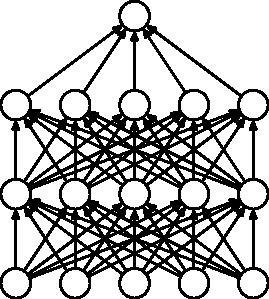
\includegraphics[width=3.5cm]{dropout-off.pdf}
		\caption{ANN}
		\label{fig:neuron}
	\end{subfigure}%
	\begin{subfigure}{.5\textwidth}
		\centering
		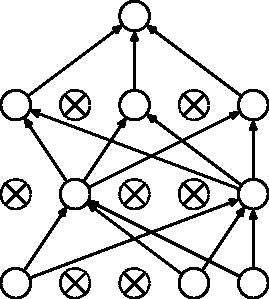
\includegraphics[width=3.5cm]{dropout-on.pdf}
		\caption{ANN na toepassing dropout}
		\label{fig:ANN}
	\end{subfigure}
	\caption{Links is een standaard ANN te zien met twee verborgen lagen, rechts is hetzelfde netwerk te zien na toepassing van dropout. De gekruiste units zijn de gedropte units.}
	\label{fig:test}
\end{figure}
\subsection{Dropout}
Tijdens het trainen kan het gebeuren dat neuronen volledig afhankelijk worden van de output van \'e\'en enkel neuron uit de vorige laag (of een kleine groep neuronen). Deze units worden lui en dragen weinig tot niets bij aan het herkenningsvermogen. Dit fenomeen heet \textit{co-adaptatie}. Om dit tegen te gaan en de units te verplichten zelf bij te dragen tot de herkenning van bepaalde patronen wordt dropout toegepast.
\npar Tijdens elke iteratiestap van het trainingsalgoritme worden een aantal units uitgeschakeld (vandaar de benaming dropout). Of een unit al dan niet wegvalt wordt bepaald door een probabiliteit \textit{Bernoulli(p)}. Deze $p$ is een hyperparameter van het netwerk en wordt doorgaans ingesteld op 0.5 waardoor getraind wordt met de helft van de units. Elke iteratiestap wordt een andere deelverzameling neuronen getraind, in essentie een ander netwerk. Het uitschakelen van units gebeurt enkel tijdens training, daarom worden de gewichten herschaald tijdens het trainen met een factor $1/(1-p)$. De niet geschaalde gewichten zijn bruikbaar in de testfase wanneer alle neuronen worden benut.
\npar Dropout is een regularisatiemethode die ondanks zijn simpliciteit erg effici\"ent blijkt. \cite{dropout} geeft een uitvoerige analyse en vergelijkende studie van het gebruik van dropout bij het uitvoeren van taken zoals gensplitsing, spraak-, tekst- en beeldherkenning. In elke van deze experimenten zorgt dropout voor een hogere regularisatie. Zo wordt aangetoond dat dropout overfitting kan tegengaan in om het even welk toepassingsgebied.

\section{Convolutioneel neuraal netwerk}
De machine learning techniek die sinds 2012 in de belangstelling staat is die van het convolutioneel neuraal netwerk. Mede dankzij het recordbrekende resultaat van \cite{cnn-krizhevsky} op de ``ImageNet Large Scale Visual Recognition Challenge'' wordt deze techniek vaak onderzocht en toegepast op beeldherkenningsproblemen zoals in \cite{cnn-ji} en \cite{cnn-karpathy}.
\npar Traditionele beeldherkenningstechnieken zoals in \cite{perronnin2010improving} en \cite{jhuang2007biologically} leiden het beeld af naar een manueel ontworpen beeldrepresentatie. Deze kenmerken zijn niet meteen zichtbaar maar worden via verschillende bewerkingen blootgelegd. Het is erg moeilijk om te beslissen welk soort kenmerk het best geschikt is voor de gegeven taak. Vaak moet er dan ook veelvuldig ge\"experimenteerd worden met verschillende representaties.
\begin{figure}[!t]
	\centering
	%	\def\svgscale{0.85}
	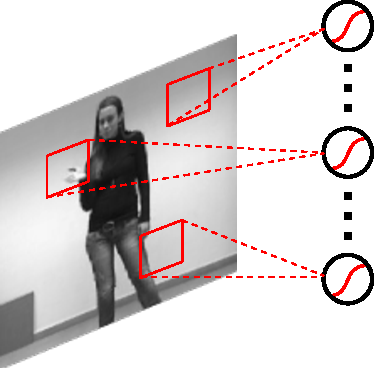
\includegraphics[width=4cm,keepaspectratio]{lokale-connectiviteit.pdf}
	\caption{Lokale connectiviteit van receptieve velden. Voor elk overlappend deelgebied van de invoer is er een neuron verbonden. Alle gewichten van het lokale filter worden gedeeld.}
	\label{fig:lokale-connectiviteit}
\end{figure}
\npar Convolutionele neurale netwerken hebben als grote troef dat ze deze feature-extractie automatiseren. Een CNN is een biologisch ge\"inspireerd model. Het onderzoek van \cite{hubel1968receptive} gaf een verklaring voor de manier waarop zoogdieren, specifiek de kat en de aap, de wereld rondom zich visueel waarnemen. De neuronen in de visuele cortex hebben een complexe laagsgewijze architectuur. Elke cel reageert op prikkels in een deelgebied van het gezichtsveld. Deze receptieve velden overlappen gedeeltelijk en bedekken zo het volledige zicht.

\npar Het herkenningsvermogen van de mens is nog altijd ontegensprekelijk veel hoger dan om het even welk artificieel herkenningssysteem. Vandaar dat er geprobeerd wordt de functionaliteit van de visuele cortex na te bootsen met een CNN. 
\npar CNN's zijn een speciaal soort meerlagig neuraal netwerk. Net zoals een ANN worden ze getraind met behulp van een back-propagation algoritme zoals beschreven in Sectie \ref{sec:leren}. Waarin een CNN verschilt is zijn architectuur. Een ANN is volledig verbonden met zijn invoer. Als we een afbeelding van 64x64 pixels rechtstreeks als invoer in een ANN willen gebruiken moeten er per knoop 4096 gewichten worden getraind. De artifici\"ele neuronen in een CNN werken net zoals de receptieve velden in de visuele cortex.

\npar Zoals te zien in Figuur \ref{fig:lokale-connectiviteit} wordt elk (mogelijk overlappend) deelgebied verbonden met een neuron. De parameters van deze verbindingen worden gedeeld tussen alle units. Zo leert het netwerk een bepaalde feature detecteren om het even waar in het beeld en zijn er slechts een beperkt aantal te trainen gewichten.
 \begin{figure}[!t]
 	\centering
 	%	\def\svgscale{0.85}
 	\def\svgwidth{0.55\columnwidth}
 	\input{figuren/convolutie.pdf_tex}
 	\caption{Tweedimensionale convolutie met een 3x3 filter.}
 	\label{fig:conv}
 \end{figure}
\npar In een CNN worden convolutielagen afgewisseld met pooling lagen. Zo worden er meerdere lagen na elkaar geplaatst om een diepe architectuur te verkrijgen. In de eerste lagen zullen basiskenmerken van laag niveau gedetecteerd worden en naarmate we dieper in het netwerk gaan worden geavanceerdere kenmerken van hoger niveau ge\"extraheerd. Zo zullen de eerste lagen features zoals randen detecteren die dan dieper in het netwerk worden samengesteld tot bijvoorbeeld een bepaalde handvorm.

\subsection{Tweedimensionale convolutie}

De receptieve velden delen hun parameters en zoeken dus naar hetzelfde kenmerk in een beeld. Ze filteren het beeld met behulp van een tweedimensionale discrete convolutie die als volgt kan worden beschreven:

\begin{equation}\label{eq:conv}
(w * x)_{h,b} = \sum_{b'=-\infty}^{+\infty}\sum_{h'=-\infty}^{+\infty} f_{b',h'}x_{b-b',h-h'}
\end{equation}

\npar met w de filterwaarden en x de invoer. De grootte van het filter en van de invoer is uiteraard begrensd. Met onze filtergrootte $(H_f,B_f)$ en de dimensie van onze invoer $(H_x,B_x)$ kunnen we (\ref{eq:conv}) vereenvoudigen tot:

\begin{equation}
\sum_{b'=0}^{B_f}\sum_{h'=0}^{H_f} f_{b',h'}x_{b-b',h-h'}
\end{equation}

\npar Figuur \ref{fig:conv} geeft een visuele weergave van deze convolutie operatie. Op het resultaat van deze operatie wordt een niet-lineaire activatiefunctie toegepast en zo bekomen we een feature-map. Let er op dat we op de randen een probleem hebben: we krijgen te grote of te kleine indices voor de input. Om dit probleem te omzeilen zijn er twee opties: de invoer uitbreiden of enkel de convolutie berekenen wanneer alle invoerwaardes gedefinieerd zijn. Deze tweede vorm heet de \textit{echte convolutie} en wordt hier toegepast. Hierdoor is de dimensie van de uitvoer ($B_{uit},H_{uit}$) kleiner dan die van de invoer:
\begin{equation}
\begin{aligned}
B_{uit}&=B_{in}-B_f+1 \\
H_{uit}&=H_{in}-H_f+1
\end{aligned}
\end{equation}

\npar met $(B_f, H_f)$ de dimensie van de convolutiefilter. Om meerdere features te detecteren per laag worden er meerdere feature-maps gevormd om een filterbank te bekomen. Hoeveel feature-maps er per laag worden berekend is een hyperparameter van het CNN. Hier is de tweedimensionale convolutie beschreven omdat in dit onderzoek enkel met deze convolutie gewerkt wordt. Er bestaan ook driedimensionale convoluties die rekening houden met het tijdsaspect en zo spatio-temporele features extraheren.

\begin{figure}[b!]
	\centering
	%	\def\svgscale{0.85}
	%	\def\svgwidth{\columnwidth}
	\input{figuren/max-pooling.pdf_tex}
	\caption{Maximum pooling: uit elk vak in de invoer afbeelding wordt het maximum bepaald en overgenomen in de bijhorende pixel in het uitvoerbeeld.}
	\label{fig:max-pooling}
\end{figure}\textsl{\textsl{}}
\subsection{Maximum pooling}


Na de convolutielaag volgt er een pooling laag die de feature-maps opsplitst in kleine partities met een zekere pool grootte. Het maximum uit deze vensters wordt overgenomen in de uitvoer. In Figuur \ref{fig:max-pooling} wordt een max-pooling uitgevoerd met een venster van 80x80 pixels op een invoer van 400x400 pixels. Zo daalt de dimensionaliteit maar blijven de belangrijkste features behouden.
\npar De pooling operatie zorgt voor translatie-invariantie van het herkenningssysteem. Of een hand nu een paar pixels naar links, rechts, boven of onder verschuift maakt niet uit. De pooling zal al deze activaties samenbrengen tot dezelfde positie voor de volgende featuremap. 

\section{Data-augmentatie}\label{sec:data-augm}
Hoe meer data we hebben om uit te leren, hoe beter we het model kunnen generaliseren. Deze data is niet altijd beschikbaar maar kan wel artificieel gecre\"eerd worden door data-augmentatie. Door bewerkingen uit te voeren op echte voorbeelden kunnen we nieuwe beelden maken die licht vari\"eren.
\npar Zeker in het geval van one-shot learning en leren uit een minimum aantal echte voorbeelden kan data-augmentatie een grote hulp zijn. Wanneer de gebruikte voorbeelden afbeeldingen zijn, kunnen er beeldtransformaties worden uitgevoerd zoals translaties, rotaties, cropping en zooming. Er kan ook ruis toegevoegd worden en het beeld kan vervormd worden. De keuzes van gebruikte augmentatietechnieken en hun parameters zijn afhankelijk van de uit te voeren taak. 

\chapter{Uitvoering \& resultaten}
\section{Gebruikte technologi\"en}
Alle programmatie wordt uitgevoerd in Python, een dynamische \textit{high-level} programmeertaal. Python is ontwikkeld met het oog op leesbare en kernachtige code. Het is een van de meest gebruikte talen voor het uitvoeren van wetenschappelijke experimenten, mede dankzij de vele krachtige bibliotheken die beschikbaar zijn. In dit onderzoek worden de volgende Python-bibliotheken gebruikt:

\begin{itemize}
	\item NumPy: voegt ondersteuning toe voor grote, multi-dimensionale arrays en matrices samen met een groot assortiment aan wiskundige functies om deze arrays effici\"ent te  manipuleren. Deze bibliotheek is een onderdeel van de SciPy-stack (Scientific Python).
	\item Theano \cite{theano}:  een bibliotheek die toelaat wiskundige expressies te defini\"eren, optimaliseren en evalueren. De twee belangrijkste troeven van Theano zijn de dynamische generatie van c-code en het transparante gebruik van GPU-acceleratie. Expressies worden symbolisch omgezet en gecompileerd voor een snelle en effici\"ente uitvoering. Ook worden ze geoptimaliseerd  voor gebruik van de GPU.  Hiernaast biedt de bibliotheek ook heel wat functies voor machine learning. 
	\item Lasagne \cite{lasagne}: een lightweight bibliotheek voor het bouwen en trainen van neurale netwerken. Het biedt verschillende veelgebruikte kosten-, regularisatie-, activatie- en leerfuncties aan alsook vele soorten \textit{layers}. Zo gebruikt dit werk de \textit{DenseLayer} voor volledig verbonden lagen en de \textit{Conv2DLayer} voor de tweedimensionale convolutie. Deze bibliotheek bouwt verder op functionaliteit van Theano waardoor neurale netwerken gebouwd met Lasagne ook gebruik kunnen maken van GPU-acceleratie.
	\item Scikit-learn: deze bibliotheek biedt heel wat machine learning functionaliteit aan maar hiervan wordt in dit onderzoek geen gebruik gemaakt. Het pakket binnen scikit-learn dat wel gebruikt wordt, is \textit{metrics}. Deze wordt gebruikt voor de evaluatie van het model. Vanuit de voorspelde en ware labels kunnen we via diverse functies de kwaliteit van de classificatie beschouwen. Dit pakket wordt voornamelijk gebruikt voor het berekenen van de precision en recall, en het opstellen van de confusion matrix. Deze termen worden verklaard in Sectie \ref{sec:pr-conf}.
	\item Scikit-image: is een verzameling beeldverwerkingsalgoritmes. Deze bibliotheek wordt gebruikt voor de data-augmentatie.
	
\end{itemize}
\section{ChaLearn dataset}
De gebruikte dataset is die van de ``ChaLearn Looking at People Challenge 2014'' zoals beschreven in \cite{escalera_chalearn_2014}. Uit deze set wordt de derde track gebruikt: ``gesture recognition''. Deze bevat meer dan 14000 gebaren uit een vocabularium van 20 Italiaanse gebaren. Merk op dat het hier niet gaat om een gebarentaal maar om afzonderlijke gebaren uit de Italiaanse cultuur. De verschillende gebaren en hun benamingen zijn te zien in \ref{fig:gebaren}.
\begin{figure}
	\centering
	%	\def\svgscale{0.85}
	\def\svgwidth{\columnwidth}
	\input{figuren/gebaren.pdf_tex}
	\caption{De Italiaanse gebaren gebruikt in de ``ChaLearn Looking At People Challenge 2014, Track 3: gesture spotting''}
	\label{fig:gebaren}
\end{figure}
\npar De gebaren worden uitgevoerd door 27 gebruikers tegen verschillende achtergronden. Er is variatie op vlak van kleding, lichaamsbouw, belichting, gebaaruitvoering. De beelden zijn opgenomen met behulp van een Kinect camera waardoor er vier datastromen zijn: RGB-beeld, dieptebeeld, gebruikersindex en skeletinformatie (Figuur \ref{fig:chalearn-data}).
\begin{figure}
	\centering
	%	\def\svgscale{0.85}
	\def\svgwidth{\columnwidth}
	\input{figuren/chalearn-data.pdf_tex}
	\caption{De vier datastromen beschikbaar in de ``ChaLearn Looking At People Challenge 2014, Track 3: gesture spotting'' dataset}
	\label{fig:chalearn-data}
\end{figure}
\npar Deze dataset werd ook gebruikt in \cite{lionel} waar deze een aantal voorverwerkingsstappen onderging. Deze voorverwerkte dataset is ter beschikking gesteld van dit onderzoek. De voorverwerking probeert de dataset te optimaliseren voor gebarenherkenning. De dataset bestaat uit 10000 ge\"isoleerde gebaren samen met hun correcte klasselabel. Er worden 32 frames geselecteerd rond het midden van elk gebaar. Vervolgens worden er vier nieuwe datastromen gecre\"eerd door het uitsnijden van de linker en rechterhand uit zowel diepte- als RGB-beeld. Ook wordt het bovenlichaam ge\"isoleerd om een deel van de achtergrond weg te werken. In totaal zijn er zo zes datastromen beschikbaar. Elk beeld, origineel 640x480 pixels groot, wordt gedownscaled en gecropt tot een grootte van 64x64 pixels. 

\npar In dit onderzoek wordt de dataset opgedeeld in 60\% training-, 20\% validatie- en 20\% testset. Deze opdeling is sequentieel gebeurd: het eerste deel voor training, het tweede deel voor validatie en het laatste voor test.


\section{Onderzoeksopzet}

De experimenten worden uitgevoerd op computers van het Reservoir Lab aan van de vakgroep Elektronica- en Informatiesystemen (ELIS) van de Universiteit Gent. De gebruikte computers hebben een hexacore processor (Intel Core i7-3930K) met kloksnelheid van 3.2 GHz en een NVIDIA Tesla K40c grafische kaart.

\npar In een eerste fase moet er een convolutioneel neuraal netwerk worden opgezet die een aanvaardbare nauwkeurigheid behaald op de gebruikte dataset. Dit model wordt besproken in sectie \ref{sec:basismodel}. De nauwkeurigheden van dit predictief model getraind op alle klassen met alle voorbeelden wordt vervolgens gebruikt als vergelijkingspunt of \textit{baseline} voor de one-shot learning experimenten.

\npar In de volgende stap zal een model, qua architectuur en hyperparameters gelijkend op het basismodel, getraind worden op een deelverzameling van de gebaren. Na deze pre-training kan het model een gebaar bijgeleerd worden en wordt er ge\"experimenteerd met het aantal verschillende samples van het nieuwe gebaar, het aantal lagen dat hertraind worden en met het gebruik van data-augmentatie. De bespreking van deze experimenten gebeurt in sectie \ref{sec:experimenten}.

\section{Ontwerp en optimalisatie van het basismodel}\label{sec:basismodel}
Alle keuzes omtrent hyperparameters en architectuur zijn experimenteel, op basis van gelijkaardige onderzoeken en naar advies van de begeleiding bepaald. Er zijn vele mogelijke combinaties qua hyperparameters en het is zeer tijdrovend om hierin de meest optimale keuze te maken. Dit is ook niet de essentie van dit onderzoek. Er dient een voldoende goed model opgesteld te worden om vergelijkingen te maken tussen het leren van alle gebaren (basismodel) en het bijleren van een gebaar. 
\subsection{Invoer}
Uit het beeld van elk gebaar worden 4 frames gesampled per datastroom. Er is gekozen om niet van alle input gebruik te maken om een snellere trainingstijd te bekomen zodat er meer experimenten kunnen worden uitgevoerd. In een latere fase of bij verder onderzoek kan het model steeds uitgebreid worden om meer gebruik te maken van spatio-temporele data.
\npar Er wordt enkel gebruik gemaakt van het dieptebeeld, volgens \cite{lionel} en \cite{wu_deep_2014} ligt hierin de nuttigste informatie voor een CNN. Het gebruik van RGB-beeld in combinatie met grijswaardenbeeld voegt meestal weinig toe. Hierin kan dus ook weer rekentijd worden gespaard.
\begin{figure}
	\centering
	%	\def\svgscale{0.85}
	\def\svgwidth{0.5\columnwidth}
	\input{figuren/dataset-input.pdf_tex}
	\caption{De 12 frames gebruikt voor de invoer van het CNN. De frames hebben een resolutie van 64x64 pixels.}
	\label{fig:dataset-input}
\end{figure}
\npar Per voorbeeld zijn er 12 beelden zoals weergegeven in Figuur \ref{fig:dataset-input}. De input van de invoerlaag heeft dus een dimensie van 12x64x64. Merk op dat de beelden van de handen en het volledige bovenlichaam in hetzelfde CNN worden verwerkt. Alle uitgevoerde experimenten hanteren deze invoerdimensie.

\subsection{Architectuur}
\begin{figure}
	\centering
	%	\def\svgscale{0.85}
	\def\svgwidth{\columnwidth}
	\input{figuren/First-model.pdf_tex}
	\caption{Het basismodel bestaande uit een drielagig CNN voor feature-extractie en een drielagig ANN (met softmax uitvoerlaag) voor classificatie}
	\label{fig:model-1}
\end{figure}
Het opgestelde basismodel is weergegeven in figuur \ref{fig:model-1}
Het CNN bestaat uit drie convolutionele en max-pooling lagen. Alle max-pooling gebeurt met vensters van 2x2 zodat het beeld telkens gehalveerd wordt in grootte. De eerste convolutionele laag bevat 8 5x5 filters, de tweede 16 5x5 filters en de laatste 32 4x4 filters.
\npar De output van dit CNN wordt gebruikt als featurevector in een ANN voor classificatie. Het ANN bevat ook drie lagen, de twee verborgen lagen hebben respectievelijk 800 en 100 knopen. Alle verborgen knopen zijn ReLU's en aan de uitgangslaag wordt een softmax gebruikt met 20 units voor de classificatie van de verschillende gebaren.
\begin{table}
	\centering
	%	\vspace{5pt}
	\renewcommand{\arraystretch}{0.8}% 
	\begin{tabular}{ l l }
		\hline
		\textit{Hyperparameter} & \textit{Waarde} \\
		\hline
		\hline
		\textbf{Filters CNN:} & \\
		\quad Laag 1 & 8x(5x5) \\
		\quad Laag 2 & 16x(5x5) \\
		\quad Laag 2 & 32x(4x4) \\
		
		\textbf{Verborgen units ANN:} &\\
		\quad Laag 1 & 800\\
		\quad Laag 2 & 100 \\
		\hline
		Max-pooling vensters & 2x2\\
		Learning rate & $10^{-4}$\\
		Batch grootte & 32\\
		Dropout kans & 0.5\\
		Nesterov momentum & 0.9\\
		\hline
		\textbf{Initialisatie:} & \\
		Gewichten CNN & Glorot initialisatie (uit uniforme verdeling $[-a,a]$)\\
		Bias CNN & 0 \\
		Gewichten ANN & Glorot initialisatie (uit uniforme verdeling $[-a,a]$)\\
		Bias ANN & 0 \\
		\hline
		\textbf{Data-augmentatie:} & \\
		Zoom & [83.33,120] \%, uniforme verdeling \\
		Rotatie & [-2,2]$^{\circ}$, uniforme verdeling\\
		2D translatie & [-2,2] pixels, uniforme verdeling
		
	\end{tabular}	
	\caption{Hyperparameters van het basismodel}\label{tab:hyperparam}
\end{table}
\npar Een samenvatting van alle hyperparameters en gekozen architectuur is te vinden in Tabel \ref{tab:hyperparam}. Voor de regularisatie wordt er gebruik gemaakt van dropout. De gewichten worden ge\"initiaseerd met Glorot gewichten gesampled uit een uniforme verdeling. Deze gewichtsinitialisatie beschreven in \cite{glorot-1} is ontwikkeld voor deep learning methodes en de standaard initialisatiemethode van het Lasagne framework. Het zorgt ervoor dat de aangelegde invoer zich kan propageren tot diep in het netwerk. Zonder goede intitialisatie van de gewichten is er een risico dat het signaal fel afzwakt waardoor de laatste lagen geen input krijgen.
\npar Er wordt ook aan data-augmentatie gedaan om de prestatie van het predictief model te verbeteren. De parameters van deze augmentatie staan beschreven in Tabel \ref{tab:hyperparam}. Deze parameters bleken later nogal conservatief gekozen, in Sectie \ref{sec:softmax19x1} wordt hierover uitgebreid.
%De gebruikte data-augmentatie bleek bij nader inzien geen zo'n grote impact te hebben door conservatief gekozen parameters zoals weergegeven onderaan Tabel \ref{tab:hyperparam}. De parameters voor translatie en rotatie zijn eigenlijk te klein en voegen weinig variatie toe aan de beelden. In Sectie \ref{sec:model-19x1} wordt hierover verder uitgebreid.
\subsection{Training}
\npar Mini-batch gradient descent aangevuld met Nesterov Augmented Momentum worden gebruikt als optimalisatie-algoritme. Alle training wordt uitgevoerd op de GPU waardoor we de CPU kunnen gebruiken om de voorbeelden aan te voeren. Dit verloopt als volgt:
\begin{itemize}
	\item een werk-proces selecteert 32 random gekozen klasselabels
	\item per gekozen klasselabel wordt een random voorbeeld van die klasse gekozen uit de trainingset
	\item elk voorbeeld wordt geaugmenteerd met behulp van een transformatiematrix
	\item de voorbeelden worden in een array in het gedeelde geheugen geplaatst en opgehaald voor training van het model
	\item tijdens de training op deze mini-batch wordt de volgende klaargezet
\end{itemize}
Na 250 iteraties, die we verder een epoch zullen noemen, wordt het model ge\"evalueerd met de validatieset. Het minimum van de validatiefout wordt bijgehouden en telkens we een lagere waarde bereiken worden de modelparameters opgeslaan. De training stopt wanneer er na een aantal epochs geen verbetering meer te zien is in de validatiefout.

\subsection{Baseline resultaten}
Om de baseline op te stellen wordt de volledige trainingset gebruikt om de 20 gebaren van de dataset te leren classificeren. Het voorgestelde model convergeert na ongeveer 250 epochs en behaalt een totale nauwkeurigheid van 81,20 \%.

\subsubsection{Precision, recall en confusion}\label{sec:pr-conf}
\begin{figure}
	\centering
	%	\def\svgscale{0.85}
	\def\svgwidth{0.7\columnwidth}
	\input{figuren/prec+recall.pdf_tex}
	\caption{Visualisatie van de betekenis van precision en recall. Links zijn alle relevante elementen te zien die zouden moeten geselecteerd worden. Het omcirkelde gedeelte zijn de effectief geselecteerde elementen of de voorspellingen van het model}
	\label{fig:prec+recall}
\end{figure}

\npar In Figuur \ref{fig:conf-allegebaren} is de genormaliseerde confusion matrix van het basismodel te zien. De mate van verwarring valt best mee, voor alle klassen ligt de waarde op de diagonaal relatief hoog. Een aantal klassen worden wel vaak verward zoals bijvoorbeeld klasse 3 en 9 ($\sim$15 \% van klasse 3 en $\sim$20 \% van klasse 9). Ook klasse 13 en 14 worden ondanks hun relatief hoge ware voorspellingswaarde ook vaak verward ($\sim$7 \% van klasse 13 en $\sim$13 \% van klasse 14)

\begin{figure}
	\centering
	\def\svgwidth{0.9\columnwidth}
	\input{figuren/conf_alle_klassen.pdf_tex}
	\caption{Genormaliseerde confusion matrix van baseline voorspellingen van het basismodel, getraind op alle voorbeelden van alle gebaren }
	\label{fig:conf-allegebaren}
	
	\vspace{1cm}
	\begin{tabular}{l l}
		\begin{tabular}{l l l}
			\hline
			\textbf{Label} & \textbf{Precision} &
			\textbf{Recall}\\
			\hline
			0 & 84,71 \% & 77,42 \% \\
			1 & 71,17 \% & 77,45 \% \\
			2 & 81,82 \% & 80,00 \% \\
			3 & 62,04 \% & 67,00 \% \\
			4 & 92,15 \% & 93,07 \% \\
			5 & 87,04 \% & 90,38 \% \\
			6 & 84,71 \% & 77,42 \% \\
			7 & 74,59 \% & 85,05 \% \\
			8 & 93,46 \% & 93,46 \% \\
			9 & 58,54 \% & 49,48 \% \\
			\hline
		\end{tabular} & 
		\begin{tabular}{l l l}
			\hline
			\textbf{Label} & \textbf{Precision} &
			\textbf{Recall}\\
			\hline
			10 & 77,27 \% & 67,33 \% \\
			11 & 84,33 \% & 69,31 \% \\
			12 & 91,57 \% & 92,55 \% \\
			13 & 80,39 \% & 79,61 \% \\
			14 & 56,41 \% & 74,16 \% \\
			\textbf{15} & \textbf{96,88} \% & \textbf{94,90} \% \\
			16 & 91,35 \% & 92,23 \% \\
			17 & 75,27 \% & 72,92 \% \\
			18 & 90,69 \% & 83,87 \% \\
			19 & 91,51 \% & 93,27 \% \\
			\hline
		\end{tabular}	
	\end{tabular}
	\captionof{table}{Precision en recall voor de voorspellingen van het basismodel getraind op alle voorbeelden van alle gebaren.}
	\label{tab:pr-alle-klassen}
\end{figure}

\npar In Tabel \ref{tab:pr-alle-klassen} zijn alle precision en recall scores van het basismodel opgelijst. Deze scores zullen gebruikt worden als baseline voor de experimenten met het bijleren en one-shotten van een gebaar. Het zijn de waardes die we nastreven bij het hertrainen.



\section{Een gebaar bijleren}\label{sec:experimenten}

\subsection{Softmax20 model}\label{sec:softmax20}

De eerste experimenten rond het bijleren van een gebaar worden uitgevoerd op een model volledig gelijk aan het basismodel (zoals afgebeeld in Figuur \ref{fig:model-1}). Eerst wordt het model getraind met een trainingset van 19 gebaren. Als het model geconvergeerd en genoeg geregulariseerd is, zou het een aantal algemene features van een nieuw gebaar moeten herkennen.

\npar De pretraining gebeurt op een softmax van 20 units, een unit wordt dus niet gebruikt. Deze opstelling is niet bruikbaar om een dynamisch uitbreidbaar herkenningssysteem te maken omdat ze ervan uit gaat dat er slechts een gebaar zal worden toegevoegd. Het is wel een goede eerste test van het potenti\"eel van het model.

\npar Door het model te hertrainen met de trainset van 19 gebaren aangevuld met een aantal samples van het nieuwe gebaar leren we het model ook op deze klasse te activeren. Om de hyperparameters van het model te optimaliseren wordt het na elke epoch ge\"evalueerd met de volledige validatieset. Deze bevat alle beschikbare voorbeelden van het nieuwe gebaar zodat er kan gelet worden op overfitting van het model op het kleine aantal trainingsvoorbeelden.

\npar Een finale evaluatie wordt gemaakt met alle voorbeelden uit de testset. Uit de voorspelling op deze testset worden de precision en recall scores van de klasse berekend en ge\"evalueerd.

\begin{figure}
	\centering
	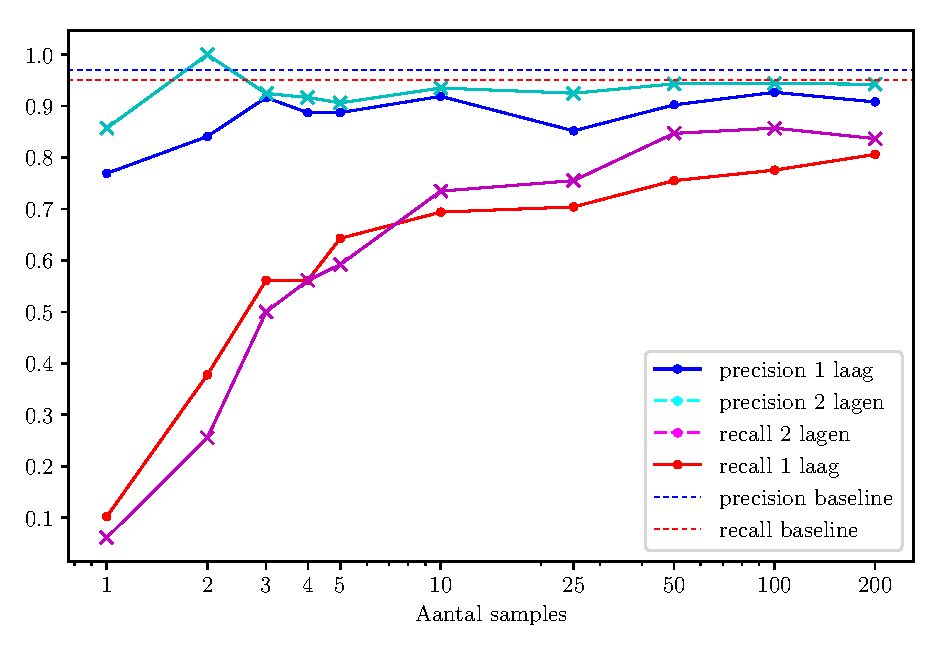
\includegraphics{naive-oneshot-lagen-vergelijking.pdf}
	\caption{Precision en recall voor de classificatie van gebaar 15 met het softmax20 model in functie van het aantal gebruikte samples voor bijleren. De streepjeslijnen geven de baseline weer van het model getrained op alle voorbeelden.}\label{fig:naive-model}
\end{figure}

\npar Eerst en vooral wordt het aantal samples gevari\"eerd. Het model wordt getraind met 200, 100, 50, 25, 10, 5, 4, 3, 2 voorbeelden en ten slotte wordt er 1 voorbeeld gebruikt voor een poging tot one-shot learning.
\npar Ook wordt het effect van het aantal hertrainde lagen onderzocht. Eerst wordt enkel de laatste laag, de softmax, hertraind. Alle andere parameters van het model blijven dus ongewijzigd. In een tweede experiment worden de softmax en de laatste verborgen laag, deze met 100 units, hertraind.

\npar In figuur \ref{fig:naive-model} zijn de resultaten van deze experimenten met het \textit{softmax20} model te zien. Het bijgeleerde gebaar is het gebaar nummer 15: "non ce ne piu". Het basismodel getraind op alle voorbeelden behaalde een 96.88\% precision en 94.90\% recall score op dit gebaar, de hoogste scores van alle gebaren. Enerzijds zou dit gebaar dus gemakkelijk moeten aan te leren zijn aangezien het heel nauwkeurig voorspeld wordt. Anderzijds kan het model zich niet meer beroepen op de features geleerd uit dit gebaar aangezien ze niet in de pretraining is opgenomen.

\npar Het is opvallend dat de precision scores voor beide experimenten heel dicht liggen bij de baseline. Het model is dus redelijk zeker dat het om het nieuwe gebaar gaat als het dit gebaar herkent. Bij het hertrainen van de twee laatste lagen met twee voorbeelden gaat de precisie zelfs boven die van de baseline.

\npar De recall score volgt niet dezelfde lijn als die van de precision. Hier zien we duidelijk dat de recall bij gebruik van weinig samples heel laag ligt. De stijlste klimming bij het model waar enkel de softmax wordt hertraind zien we tot aan het gebruik van 5 samples. Bij het hertrainen van twee lagen loopt deze stijging door tot 10 samples. Dit kan verklaard worden doordat er meer parameters geoptimaliseerd moeten worden bij het het hertrainen van de twee lagen. Meer parameters vragen om meer voorbeelden, bij gebruik van meer dan 10 samples scoort dit model dan  ook beter.

\npar Het voorgetrainde model, GARBAGE CLASS

%\npar Het opzet van dit onderzoek is zo weinig mogelijk samples te gebruiken, voor verdere experimenten werd er dus gekozen om enkel de softmax te hertrainen van het nieuwe gebaar

\subsection{Softmax19+1 model}\label{sec:softmax19x1}
We willen naar een dynamisch uitbreidbaar systeem toewerken. Het vorige model gaat uit van slechts een bij te leren gebaar en is hier dus niet bruikbaar voor. Om aan deze uitbreidbaarheid te voldoen en om verder onderzoek te voeren wordt het \textit{Softmax19+1} model opgesteld, te zien in Figuur \ref{fig:19+1model}.

\begin{figure}
	\centering
	\def\svgwidth{0.7\columnwidth}
	\input{figuren/softmax19+1.pdf_tex}
	\caption{Schematische weergave van het softmax19+1 model. De blauwe lagen zijn voorgetraind en worden niet gewijzigd. Er wordt 1 unit toegevoegd voor het nieuwe gebaar (aangeduid in het geel). De uitvoer van deze twee parallelle lagen worden samengebracht in een softmax met 20 units. Vandaar de benaming softmax19+1. }\label{fig:19x1-all}
\end{figure}

\npar Hier wordt eerst een model met 19 softmax units getraind voor de classificatie van 19 gebaren. Behalve het verschil in aantal softmax units is de architectuur volledig gelijk aan die van het basismodel. Daarna wordt het model uitgebreid met een extra unit voor de classificatie van het nieuwe gebaar. De softmax activatiefunctie van de laag met 19 eenheden wordt vervangen door een lineaire activatie ($a(x)=x$). De signalen van deze units worden samengebracht met het signaal van de nieuwe unit, ook met een lineaire activatiefunctie, in een \textit{ConcatLayer}.  Op deze laatste laag, die nu 20 eenheden telt, wordt dan de softmax uitgevoerd voor classificatie.

\begin{figure}
	\centering
	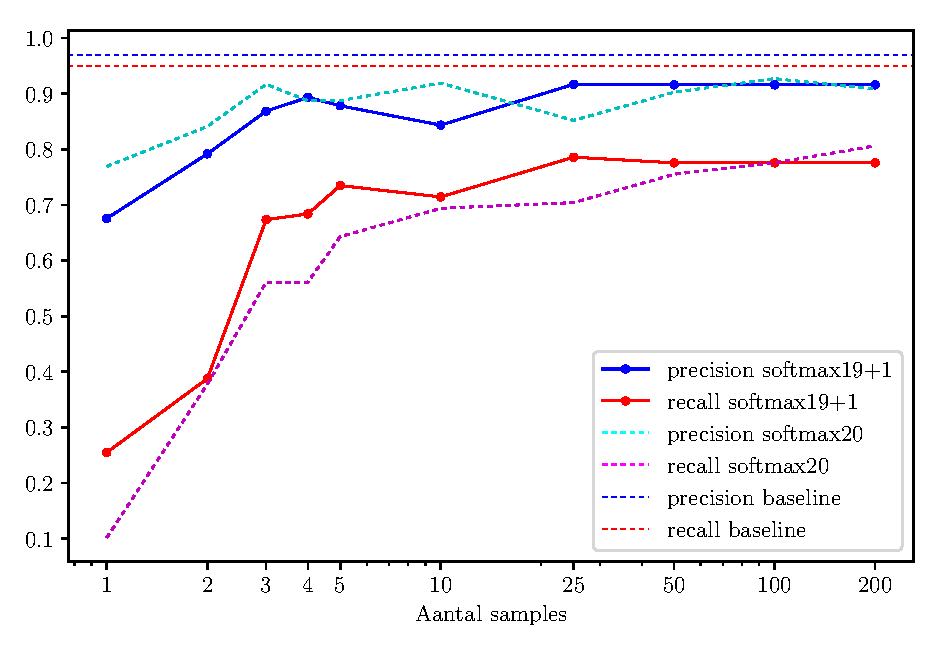
\includegraphics[width=\columnwidth]{19x1-gebaar15.pdf}
	\caption{Precision en recall voor de classificatie van gebaar 15 met het softmax19+1 model in functie van het aantal gebruikte samples voor bijleren.}\label{fig:19x1-gebaar15}
	
		\vspace{0.5cm}
		\def\svgwidth{1.1\columnwidth}
		\input{figuren/19x1-oneshot-vgl.pdf_tex}
		\caption{Barplots per gebaar van de precision en recall van de baseline en na het hertrainen met respectievelijk 1 en 10 samples. }\label{fig:19x1-all}
\end{figure}

\npar Het leren gebeurt enkel op de ene unit van het nieuwe gebaar. Aan de verborgen laag van de 19 al geleerde gebaren wordt niet geraakt zodat het herkenningsvermogen op deze gebaren gelijk blijft. Dit zal ook een vereiste zijn van een uitbreidbaar herkenningssysteem, het bijleren van een nieuw gebaar mag geen negatief effect hebben op de huidige prestatie van het model.

\subsubsection{Invloed van het aantal samples}

Het softmax19+1 model wordt getoetst tegen de prestatie van het softmax20 model. In Figuur \ref{fig:19x1-gebaar15} is de precision en recall van de classificatie van gebaar 15 te zien in functie van het aantal samples dat gebruikt wordt in de trainingset. Ook de prestatie van het softmax20 model bij hertrainen van enkel de softmax laag is geplot in streepjeslijnen. De waarden liggen niet zo heel ver uiteen. De precision van het softmax19+1 model ligt iets lager bij gebruik van minder dan 10 samples. Wel ligt de recall score globaal hoger dan die van het softmax20 model. Bij het trainen op een voorbeeld is dit 25,51 \% tegenover 10,20\%. De recall curve volgt dezelfde stijle klim tot aan het gebruik van 5 samples, tot 73,47\% waarna het nog licht stijgt bij 25 samples en dan rond de 78\% blijft.

\subsubsection{Invloed van het bijgeleerde gebaar}

De prestatie van het softmax19+1 model volgt dus dezelfde trend als die van het softmax20 model. De resultaten hier weergegeven zijn allemaal na het bijleren van gebaar 15. Welk gebaar er bijgeleerd wordt heeft uiteraard ook een invloed op de prestatie van het model. Sommige gebaren hebben vele features gemeenschappelijk met andere gebaren, andere zijn eerder uniek en zullen moeilijk herkend worden.

\npar Om een beeld te scheppen van de invloed van het bij te leren gebaar werd voor elk gebaar eerst een model getraind exclusief dit gebaar, waarna het werd bijgeleerd met 1 en met 10 samples. Op Figuur \ref{fig:19x1-all} zijn de resultaten van dit experiment te zien. Bovenaan is de precision uitgeplot van alle gebaren, onderaan de recall.

\npar De recall score na bijleren met 1 en met 10 samples volgt dezelfde lijn als die van de baseline. Gebaren die een lagere recall score hebben na trainen op alle voorbeelden van alle gebaren scoren ook lager als we ze bijleren. Hetzelfde geldt voor gebaren die hoog scoren. Zeker bij vergelijking van het gebruik van 10 samples is dit opmerkelijk.

\npar De precision volgt ook dezelfde trend maar de verschillen zijn veel kleiner. De bevindingen uit het eerste experiment op gebaar 15 zijn dus door te trekken naar de andere gebaren.

\subsubsection{Invloed van data-augmentatie}
Ten slotte wordt ook nog een experiment opgezet om de invloed van data-augmentatie te onderzoeken. Tot voor dit experiment werd data-augmentatie toegepast met de parameters beschreven in Tabel \ref{tab:hyperparam}. Nieuwe testen worden opgezet die geen augmentatie gebruiken en hier is duidelijk dat de augmentatie weinig tot geen effect heeft. De gekozen parameters blijken erg conservatief en brengen te weinig variatie in de data. Er wordt geprobeerd om een meer drastische data-augmentatie toe te passen. Om met de grotere variatie om te kunnen gaan moet het aantal parameters van het model verhoogd worden. Dit is uitgetest met een model met het dubbele aantal filterbanken in de convolutielagen en twee maal 512 units in de verborgen lagen van het ANN. Na analyse blijkt het model te underfitten: het is nog niet complex genoeg om de geaugmenteerde data te beschrijven. Om deze opstelling te optimaliseren dient er opnieuw een iteratief proces van hyperparameteroptimalisatie aangevat te worden. Hier is niet verder op ingegaan, het gebruik van data-augmentatie kan wel verder onderzocht in toekomstig werk.

\subsection{Softmax18+1+1 model}

Om de uitbreidbaarheid verder te onderzoeken wordt analoog aan het principe van het softmax19+1 model een architectuur gemaakt dat twee gebaren na elkaar bijleert. Eerst wordt een model met 18 softmax units getraind. Na deze pretraining wordt er een unit voor het bij te leren gebaar toegevoegd en net zoals het vorige model worden de uitgangen van de 18 units en de nieuwe unit samengevoegd met een ConcatLayer.
\npar Het model leert een gebaar bij door de training van het nieuw toegevoegde unit en wordt daarna opnieuw uitgebreid met nog een extra unit voor het tweede gebaar. Ook deze unit wordt geconcateneerd zodat er uiteindelijk een softmax van 20 units is (18+1+1).

\npar Door op deze manier te werk te gaan is het theoretisch mogelijk om gebaren te blijven toevoegen. Na het toevoegen van een aantal gebaren kunnen de units effectief samengevoegd worden tot een laag waarna het proces opnieuw kan beginnen.

\npar In Figuur \ref{fig:18x2} zijn de resultaten te zien van het bijleren van gebaar 13 en gebaar 18. Eerst wordt gebaar 13 bijgeleerd, daarna gebaar 18, telkens met even veel voorbeelden. De recall score van beide gebaren ligt hoger dan wanneer ze elk afzonderlijk worden bijgeleerd in het softmax19+1 model. De precision ligt dan wel weer lager, vooral bij gebaar 13 dat eerst werd aangeleerd.

\npar Waarom de recall hoger ligt dan bij het softmax19x1 model valt moeilijk te verklaren. Het bijleren van een gebaar blijkt in al de experimenten erg afhankelijk van welk gebaar wordt bijgeleerd en uit welke gebaren wordt voorgeleerd. Om dit verder uit te zoeken zouden er meer experimenten met andere gebaren moeten worden uitgevoerd.

\npar Figuur \ref{fig:conf-18x2} geeft de genormaliseerde confusion matrix weer van het bijleren uit een voorbeeld. Hierop is te zien dat er een kleine verwarring is tussen de twee nieuw aangeleerde gebaren: 6\% van gebaar 18 wordt verward met 13 en omgekeerd 3\%. De grootste verwarring bij gebaar 18 is met gebaar 14: 31\%. In het baseline model is dit ook de grootste mate van verwarring bij gebaar 18 (6\%, te zien in Figuur \ref{fig:conf-allegebaren}).


\begin{figure}
	\centering
	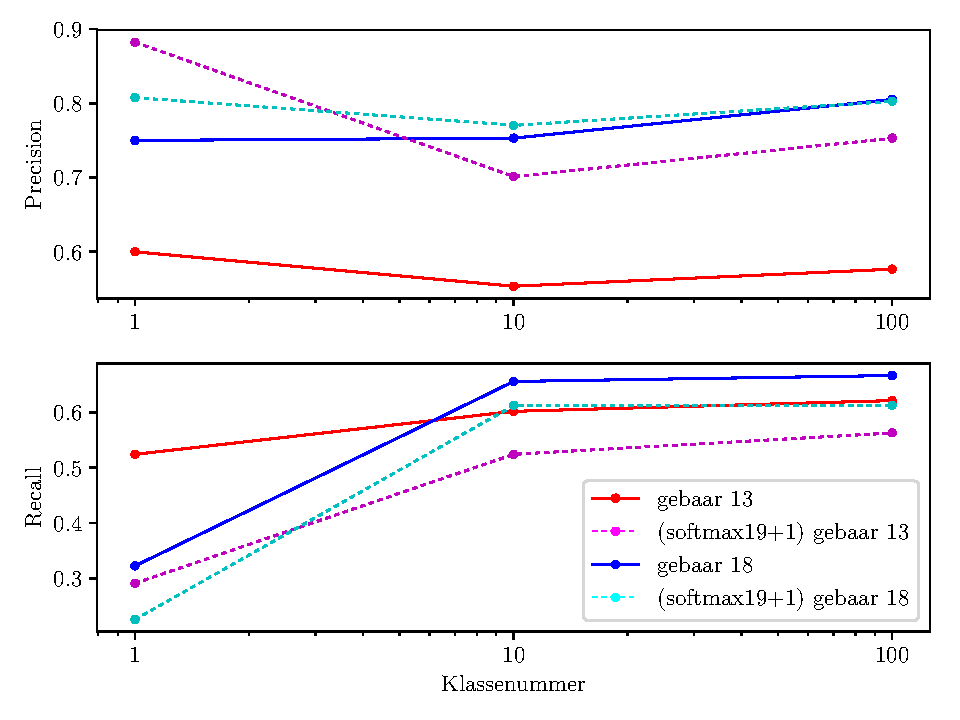
\includegraphics[width=0.90\columnwidth]{18x2.pdf}
	\caption{Precision en recall na het bijleren van gebaar 13 en gebaar 18 in het \textit{softmax18+1+1} model. Ter vergelijking is het resultaat van het \textit{softmax19+1} model ook uitgetekend.}\label{fig:18x2}
	\vspace{1.5cm}
	\def\svgwidth{0.7\columnwidth}
	\input{figuren/conf-18x2.pdf_tex}
	\caption{Genormaliseerde confusion matrix van het \textit{softmax18+1+1} model na leren van gebaar 13 en gebaar 18 met een voorbeeld.}\label{fig:conf-18x2}
\end{figure}
\chapter{Simulatieresultaten}
\label{resultaten}

\section{Wijzigingen aan de implementatie}
\label{wijzigingen}
\subsection{Het kickstartprobleem}
\npar In principe zou bovenstaande uitwerking moeten werken.  Helaas, dit was buiten ns-click gerekend waarin blijkbaar enkele rare implementatiekeuzes gemaakt werden of waar gewoon nog een aantal bugs in zitten.  Zo hadden we de rare situatie dat wanneer de dispatcher ge�mplementeerd was zoals het hoort en het downstreamverkeer dus geblokkeerd werd totdat een upstreampakket ontvangen werd, het geheel niet werkte.  Pas vanaf 3.1~s kon het eerste upstreampakket verzonden worden.  Wanneer we de dispatcher initialiseren, en deze vanaf het begin downstreamverkeer doorlaat naar een vooraf gekozen RAU, werkt alles naar behoren.  Althans zo lang de trein zich ter hoogte van de eerste RAU bevindt.  Vanaf er overgeschakeld wordt op de tweede RAU, geraakt er slechts 10\% van het upstreamverkeer meer verzonden, terwijl er voor het downstreamverkeer geen probleem is.  We hebben geen idee hoe dit komt, maar de kans bestaat dat de oorzaak in dezelfde richting moet gezocht worden als deze die problemen heeft bij de eerste RAU wanneer de dispatcher oorspronkelijk al het verkeer blokkeert.  Dit probleem werd reeds aangebracht als het \textit{kickstartprobleem} in sectie \ref{nsclick}.

\subsection{Verwisselen AP- en station-functionaliteit}
\npar Zoals uit bovenstaande paragraaf blijkt, moet het eerste verkeer afkomstig zijn van het AP.  Echter, als we aan het principe willen vasthouden dat het eerste verkeer afkomstig moet zijn van de trein, dan lijkt de conclusie eenvoudig: plaats het AP op de trein en laat de centrale voor draadloze client doorgaan.  In wezen mag dit geen verschil maken aangezien we toch met ��n station per AP werken.  Station en AP vormen samen niet meer dan een tunnel waardoor gewoon ethernet- of IP-verkeer gestuurd kan worden.  Het enige verschil is dat het AP normaal beacon frames verstuurt en dat het station zich moet authenticeren en associ�ren met het AP.  Bovendien levert dit een bijkomend voordeel op.  Om een goede werking mogelijk te maken, moet de trein regelmatig verkeer naar de centrale sturen.  Indien er geen verkeer voorhanden is, gingen we random informatie versturen.  Als de trein echter beacon frames uitzendt, dan hebben we meteen een periodieke bron van verkeer en moet daar ook niets meer voor voorzien worden.

\npar Na het verwisselen van de AP- en station-functionaliteiten blijkt alles naar behoren te werken.  Het verkeer start, met de correcte dispatcher, onmiddellijk ipv na 3.1~s en er zijn geen problemen meer nadat op een nieuw RAU werd overgegaan.  De bespreking van de resultaten is dan ook van toepassing op deze kleine ingreep, die hoegenaamd niets verandert aan de werking van het geheel buiten deze simulatie-omgeving.

\section{Referentie}
\npar Vooraleer over te gaan tot een gedetailleerde bespreking van de resultaten, is het best eerst over referentiewaarden te beschikken van een klassiek systeem.  Het is onzinnig om een vrijwillige handover als basis voor onze vergelijking te nemen.  Dit is immers afhankelijk van de implementatie van het mechanisme dat bepaalt wanneer het signaal van het oude AP te zwak wordt en dat van het nieuwe sterk genoeg geworden is, en er tot een handover overgegaan wordt.  Bovendien wacht een standaard client nog op een ACK-bericht na het sturen van de disassociate, wat bij een slecht signaal wel heel lang kan duren na enkele retries.  In onze simulaties beslissen we zelf wanneer we overschakelen en is het signaal tijdens het overschakelen altijd goed genoeg.  Van zodra we de handover uitgevoerd hebben, wordt het signaal enkel nog beter.  We vergelijken dus best met een test met gedwongen handovers, waarbij we zelf beslissen om het station te laten associ�ren met een nieuw AP terwijl de signaalkwaliteit van beide AP's constant blijft op een goede waarde.  Testresultaten met gedwongen handovers op het goede moment leveren betere resultaten op dan wanneer de beslissing overgelaten wordt aan het station dat geen idee heeft waar het zich bevindt en welk signaal er sterker of zwakker zal worden.  Als ons systeem even goed of beter scoort dan een vergelijkbaar systeem met gedwongen handovers, dan weten we ook waar we staan ten opzichte van de situatie met door het station ge�nitieerde handovers.

\subsection{Hardwaretest}
\npar Een eerste test waarmee we kunnen vergelijken, is een hardwaretest die deze zomer uitgevoerd werd tijdens een stage.  Hiervoor hernemen we grafieken C.8 en C.9 van pagina's 43 en 44 van het stageverslag \cite{stage} over als figuren \ref{Chantry1} en \ref{Chantry2}.  Beiden zijn het resultaat van het sturen van een UDP-teststroom van +/-~1~Mbps vanaf een server in het bovenliggend netwerk naar het station.  Figuur \ref{Chantry2} is een detailopname van de handover.  5~s na het begin van de datastroom werd tot een handover overgegaan, die duidelijk te herkennen is aan de \textit{gap} van +/-~300~ms in de grafiek gedurende dewelke geen verkeer door de draadloze brug mogelijk was.  De AP's zijn Chantry Beaconpoints, die sinds de overname door Siemens door het leven gaan als Siemens HiPath.  Het station is een door Linux aangedreven laptop met Intel IPW2200 interne WiFi-kaart.

\begin{figure}[ht]
  \begin{center}
    \includegraphics[width=.5\textwidth]{Chantry1.png}
    \caption{Analyse van een UDP-teststroom aan +/-~1~Mbps met na de $26^e$ seconde (5~s na het begin van de datastroom) een handover.  De horizontale as is de tijdsas, verticaal staat de doorstroom in \textit{Bytes per tick}.  E�n tick is 0,1~s waardoor de waarde 10.000 op de grafiek overeenkomt met 100.000~Bps of 800~Kbps.\label{Chantry1}}
  \end{center}
\end{figure}

\begin{figure}[ht]
  \begin{center}
    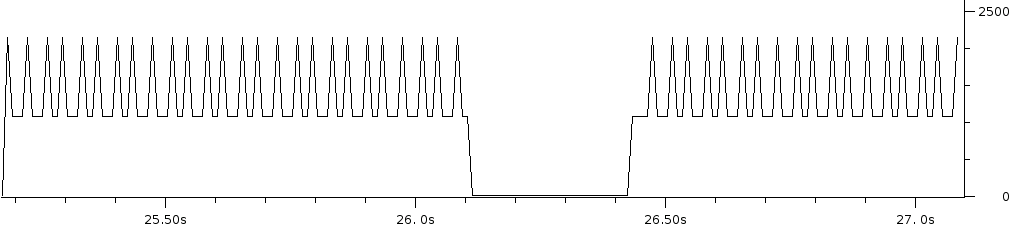
\includegraphics[width=\textwidth]{Chantry2.png}
    \caption{Detail van de handover van figuur \ref{Chantry1}: tijdens een UDP-teststroom aan +/-~1~Mbps werd na de $26^e$ seconde (5~s na het begin van de stroom) tot een handover overgegaan.  De horizontale as is de tijdsas, verticaal staat de doorstroom in \textit{Bytes per tick}.  E�n tick is 0,01~s waardoor de waarde 1.000 op de grafiek overeenkomt met 100.000~Bps of 800~Kbps.\label{Chantry2}}
  \end{center}
\end{figure}

\npar Bij deze vergelijkingsbasis dienen uiteraard de nodige kritische bedenkingen aangebracht te worden.  Deze hardwaresimulatie werd uitgevoerd op een platform dat ontwikkeld werd voor snelle handovers.  Bovendien werd hier gewerkt met de IEEE~802.11g standaard in plaats van de b-standaard die wij gebruiken.  Verder is ns-click echt niet geschikt voor doorstroomtesten aangezien er een beperking zit op de verkeersstroom die men met ns door een draadloze brug kan sturen.

\subsection{Simulatie met conventionele AP's in ns-click}
\label{resultaten-simulatie-ap}
\npar Een betere basis om mee te vergelijken, zou het nabootsen van een klassieke situatie zijn in ns-click.  Op die manier worden simulatieresultaten afkomstig van dezelfde simulator, met dezelfde eigenschappen en beperkingen, met elkaar vergeleken.  Dit is echter ook niet evident.  De modellen voor een AP en station die gebruikt worden in ns-click zijn slechts basismodellen.  De standaard wordt (grotendeels) gevolgd, maar het blijft toch mogelijk om pakketten te versturen over de draadloze brug ook zonder dat het station geassocieerd is met het AP.  Een voorbeeld van een dergelijke gecapteerde pakketstroom is te vinden in \ref{details-pakketstroom}.  Als het station overschakelt op een nieuw AP, dan kan deze al onmiddellijk upstreampakketten sturen via het nieuwe AP, nog voor het geassocieerd is, waarna de bovenliggende switch onmiddellijk de downstreampakketten naar het nieuwe AP stuurt.  De pakketten in de buffers van het oude AP gaan dan verloren, tenzij deze door de node in het bovenliggend netwerk opnieuw verstuurd worden.  Indien het station geen verkeer naar een node in het bovenliggende netwerk stuurt, zal de switch ook nooit weten dat het station bereikt moet worden via een nieuw AP en zullen de pakketten nog steeds enkel bij het oude AP toekomen alwaar ze de buffers laten overlopen en verloren gaan. In bovenstaande hardwaretest gaan geen pakketten verloren: het oude AP stuurt deze naar het nieuwe AP via het Inter Access Point Protocol (IAPP), dat momenteel gestandaardiseerd wordt, of via een eigen IAPP.  Het is echter niet omdat men direct pakketten kan versturen na het overschakelen op een nieuw AP, dat er geen handovertijd zou zijn.  Het omschakelen op een nieuwe frequentie en het synchroniseren met een zender op die frequentie vergt ook enige tijd.

\begin{figure}[ht]
  \begin{center}
    \includegraphics[width=.75\textwidth]{2ap}
    \caption{Testopstelling voor het bepalen van een vergelijkingsbasis.\label{2ap}}
  \end{center}
\end{figure}

\npar Er werd een testopstelling aangemaakt in ns-click zoals afgebeeld in figuur \ref{2ap}.  De nodes zijn vast gepositioneerd op de opgegeven co�rdinaten.  Na 1~s stelt het station zich in op kanaal~1 en authenticeert het zich bij AP0 om 10~ms later ermee te associ�ren.  2~s na het begin van de simulatie wordt een UDP-teststroom aan een bitrate van 3,6 Mbps gestuurd van de server naar het station.  100~ms later begint een gelijkaardige bitstroom in de omgekeerde richting.  Na 2~s verandert het station naar kanaal~6 om zich te authenticeren bij AP1.  Dat er ondertussen al pakketten gestuurd worden, is af te lezen in bijlage \ref{details}: gedetailleerde resultaten.  De simulatie wordt afgebroken na 6~seconden.  De resultaten zijn grafisch uitgezet in figuur \ref{referentie}.  De zwarte lijn stelt de totale doorstroom door de draadloze link voor.  Groen en rood staan voor de stroom van het station naar de server, respectievelijk van de server naar het station.  Er is duidelijk een gap te zien op het moment dat overgeschakeld wordt op de nieuwe frequentie.  Dit moment is uitvergroot in figuur \ref{referentie-detail}.  Deze gap is 100~ms breed voor de rode lijn en 90~ms voor de andere lijnen.  Dit verschil is te verklaren door het feit dat pas vanaf het eerste upstream UDP-pakket de switch bereikt heeft, deze overschakelt en aankomende downlink UDP-pakketten naar het nieuwe AP stuurt.

\begin{figure}[ht]
  \begin{center}
    \includegraphics[width=.75\textwidth]{referentie}
    \caption{Doorstroom van een UDP-teststroom bij 2 gewone AP's.  De horizontale as is de tijdsas, verticaal staat de doorstroom in \textit{Bytes per tick}.  E�n tick is 0,1~s waardoor de waarde 100.000 op de grafiek overeenkomt met 1.000.000~Bps of 8~Mbps.\label{referentie}}
  \end{center}
\end{figure}


\begin{figure}[ht]
  \begin{center}
    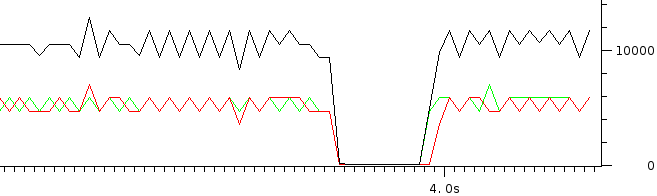
\includegraphics[width=.75\textwidth]{referentie-detail}
    \caption{Detailopname van de handover tijdens de doorstroom van een UDP-teststroom bij 2 gewone AP's, zoals weergegeven in figuur \ref{referentie}.  De horizontale as is de tijdsas, verticaal staat de doorstroom in \textit{Bytes per tick}.  E�n tick (hier ��n klein streepje op de horizontale as) is 0,01~s waardoor de waarde 10.000 op de grafiek overeenkomt met 1.000.000~Bps of 8~Mbps.\label{referentie-detail}}
  \end{center}
\end{figure}

\section{Resultaten van het systeem op basis van Radio-over-Fiber}
\npar Zoals vermeld in \ref{werking-systeem}, is dit een uiterst flexibel systeem.  Meerdere (kruisende) treinen, meerdere kanalen per trein, er is heel wat mogelijk.  We zullen in deze sectie een paar van deze voorbeelden uitwerken en de simulatieresultaten bespreken.  We beginnen uiteraard bij een basisgeval om de werking van het moving cell principe te illustreren.

\subsection{1 trein, 2 remote antenna units}
\label{1t2bs}
\npar De testopstelling is ge�llustreerd in figuur \ref{1trein2bs}.  Het bereik van de draadloze nodes is afgesteld op 105~m, zodat we een overlapzone van 10~m bekomen.  Het grote voordeel aan deze manier van werken, is dat wanneer er overgeschakeld wordt op een nieuwe RAU, eventuele data die nog onderweg is van de centrale naar de oude RAU alsnog afgeleverd kan worden op de trein.  De trein is ondertussen overgeschakeld op de nieuwe RAU en de signaalkwaliteit zal alleen maar verbeteren, tot wanneer de trein de RAU voorbijrijdt.

\begin{figure}[ht]
  \begin{center}
    \includegraphics[width=.75\textwidth]{1trein2bs}
    \caption{Testopstelling met 1 trein en 2 RAU's.\label{1trein2bs}}
  \end{center}
\end{figure}

\npar Initieel staat de trein stil op de beginpositie.  Het AP in de trein is reeds actief vanaf het begin en zendt op regelmatige tijdstippen beacon frames uit.  Na 1~s gaat het station in de centrale een probe request uitsturen naar het AP dat zich op de trein bevindt, van waaruit een antwoord teruggestuurd wordt.  500~ms later authenticeert het station zich, om 100~ms later te associ�ren met het AP.  2~seconden na het begin van de simulatie, start de trein zijn beweging aan 40~m/s, wat overeenkomt met 144~km/u.  Op seconde 3 start vervolgens een bitstroom aan 3,6~Mbps van de server naar de trein.  Om een nog onbekende reden is de troughput van de trein naar de centrale bijzonder laag.  De omgekeerde richting, van de server naar de trein, is echter het interessantst van al.  Het is deze stroom die naar de juiste RAU gerouteerd moet worden om op de trein terecht te komen.  Aan de trein zelf verandert er niets: het is steeds hetzelfde station (in de centrale) dat geassocieerd blijft met het AP in de trein en deze laatste verandert ook niet van frequentie of andere parameters.  Enkel in de centrale gebeurt de omschakeling naar de nieuwe RAU.  Na 8~s is het experiment voorbij.

\npar Een analyse van de bitstroom levert bijzonder interessante informatie op.  Het resultaat is grafisch weergegeven in figuur \ref{resultaten-1t2bs}.  In tegenstelling tot de referentiemetingen is hier helemaal geen gap of dipje te merken in de doorstroom.  De stroom is continu.

\begin{figure}[ht]
  \begin{center}
    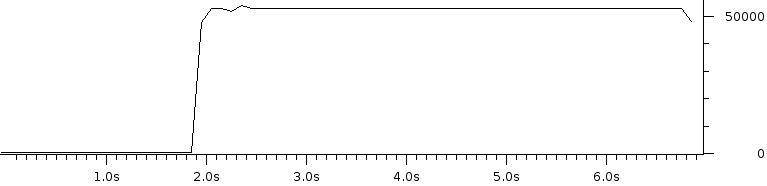
\includegraphics[width=.75\textwidth]{resultaten-1t2bs}
    \caption{Doorstroom van een UDP-teststroom bij het RoF-model.  De horizontale as is de tijdsas, verticaal staat de doorstroom in \textit{Bytes per tick}.  E�n tick is 0,1~s waardoor de waarde 50.000 op de grafiek overeenkomt met 500.000~Bps of 4~Mbps.\label{resultaten-1t2bs}}
  \end{center}
\end{figure}

\npar Een ander interessant experiment, is het meten van de bitstroom aan de centrale, meerbepaald het verkeer van en naar de RAU's.  Als we dat verkeer opsplitsen per RAU, zien we hoe lang de trein zich in de overlapzone bevindt en wanneer de centrale omgeschakeld is naar de nieuwe RAU.  Om een en ander beter zichtbaar te maken, sturen we ook een kleine UDP-teststroom van 76~kbps van de trein naar de server.  Op die manier hebben we iets meer verkeer en bekomen we kwalitatievere metingen.  De resultaten zijn te zien in figuur \ref{RoF-1t2rau-centrale}.  We zien dat vanaf het eerste pakket van de tweede RAU (paarse lijn) binnenkomt op seconde 4,35, de centrale overschakelt en het verkeer naar RAU0 (de rode lijn) volledig naar nul gaat.  Op de grafiek lijkt dit niet onmiddellijk te gaan, maar ongeveer 200~ms te duren.  Dit klopt niet: dit zou moeten een rechte verticale lijn zijn.  Dit is beter zichtbaar in een detailopname van de handover, weergegeven in figuur \ref{RoF-1t2rau-centrale-detail}.  De trein bevindt zich in de overlapzone als de uitgezonden pakketten opgepikt worden door zowel RAU0 en RAU1, wat op de grafiek te zien is als de zone waar de paarse en blauwe lijn samen verschillen van nul.  Dit is het geval vanaf 4,3~s tot 4,75~s.  De centrale is echter al vanaf het begin overgeschakeld, daar waar de groene lijn (het verkeer naar RAU1) de tijdsas verlaat.  Er is duidelijk te zien dat het verkeer, zowel van de server naar de trein als omgekeerd, niet onderbroken wordt.

\npar Figuur \ref{RoF-1t2rau-centrale-detail} lijkt grilliger, wat komt door de sterke uitvergroting van de tijdschaal.  Elke lage piek komt dan overeen met een binnenkomend of vertrekkend pakket, UDP-pakketten worden verzonden met een datainhoud van 1000 bytes.  Hier is de omschakeling van de centrale op RAU1 beter te zien: de rode en groene lijn zijn steiler en het gebied waar beiden van de tijdsas afwijken, is in verhouding tot de overlapzone (waar de blauwe en paarse lijn van de tijdsas afwijken) veel kleiner dan op figuur \ref{RoF-1t2rau-centrale}, wat duidelijk aangeeft dat de breedte van de groen-rode overlap een zuiver grafische oorzaak heeft.

\begin{figure}[ht]
  \begin{center}
    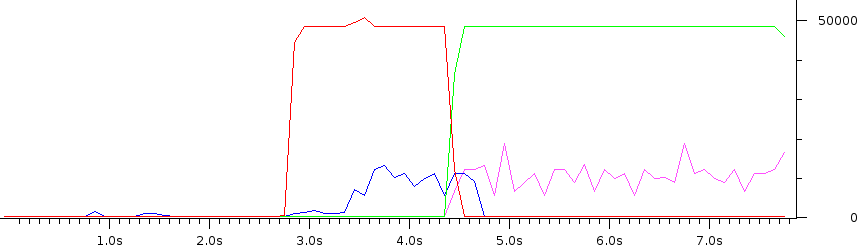
\includegraphics[width=.9\textwidth]{RoF-1t2rau-centrale.png}
    \caption{Pakketstromen tussen de centrale en de RAU's in het RoF-model.  De horizontale as is de tijdsas, verticaal staat de doorstroom in \textit{Bytes per tick}.  E�n tick is 0,1~s waardoor de waarde 50.000 op de grafiek overeenkomt met 500.000~Bps of 4~Mbps.  De rode en groene lijnen geven het verkeer van de centrale naar RAU0, respectievelijk RAU1, weer, terwijl de blauwe en paarse lijnen de stroom van RAU0 respectievelijk RAU1 naa de centrale voorstellen.\label{RoF-1t2rau-centrale}}
  \end{center}
\end{figure}


\begin{figure}[ht]
  \begin{center}
    \includegraphics[width=.9\textwidth]{RoF-1t2rau-centrale-detail.png}
    \caption{Detailopname van de pakketstromen tussen de centrale en de RAU's in het RoF-model.  De horizontale as is de tijdsas, verticaal staat de doorstroom in \textit{Bytes per tick}.  E�n tick is 0,01~s waardoor de waarde 5.000 op de grafiek overeenkomt met 500.000~Bps of 4~Mbps.  De rode en groene lijnen geven het verkeer van de centrale naar RAU0, respectievelijk RAU1, weer, terwijl de blauwe en paarse lijnen de stroom van RAU0 respectievelijk RAU1 naar de centrale voorstellen.\label{RoF-1t2rau-centrale-detail}}
  \end{center}
\end{figure}


\subsection{2 treinen, 3 remote antenna units}
\label{2t3bs}

\npar Zoals reeds meermaals in dit werk vermeld, is ons model bijzonder flexibel.  Er kunnen meerdere kruisende treinen zijn, of treinen die behoefte hebben aan een hogere bandbreedte, kunnen een bijkomend kanaal toegewezen krijgen.  Uiteraard is het aangewezen ook dit even experimenteel na te gaan.  Hiervoor cre�ren we een opstelling zoals weergegeven in figuur \ref{2trein3bs}.  Wanneer we naar beide treinen afzonderlijk maar simultaan een teststroom willen sturen van 3,2~Mbps, komen we al snel een beperkende factor tegen.  Na +/-~7~seconden, als de eerste trein zich in het overlapgebied van RAU0 en RAU1 bevindt en de tweede in dat van RAU1 en RAU2, loopt de eerste wachtlijn in een RAU reeds over, namelijk deze aan de vaste netwerkverbinding van RAU1 die 10 pakketten kan bevatten.  Dit is vrij logisch: de centrale en de RAU's bevinden zich in onze opstelling in ��n collision domain, en als de treinen zich in het overlapgebied bevinden, worden hun signalen telkens door twee RAU's opgevangen en naar de centrale gestuurd.  Bij een re�le uitvoering zou dit niet mogen voorvallen.  Daar heeft elke RAU immers een directe link naar de centrale die niet met andere RAU's gedeeld wordt en bovendien up- en downlinkverkeer gescheiden houdt.

\begin{figure}[ht]
  \begin{center}
    \includegraphics[width=\textwidth]{2trein3bs}
    \caption{Testopstelling met 2 treinen en 3 RAU's.\label{2trein3bs}}
  \end{center}
\end{figure}

\npar Het is geweten dat het met ns redelijk moeilijk is om throughputmetingen te doen.  Echter, het belangrijkste doel in dit werk is het demonstreren van het concept \textit{moving cell} en de mogelijkheden ermee.  Wanneer we de bitrate van de UDP-teststromen verminderen, lopen de wachtlijnen dan ook niet meer over.  Als we nu bij elke trein individueel gaan kijken naar de doorstroom, dan levert dat gelijkaardige figuren op als in de vorige sectie met ��n trein, alleen ligt de bitrate lager.  Een interessantere meting om het concept te illustreren, bestaat er weer in om de pakketten op de link tussen de centrale en de RAU's te meten.  Een dergelijke meting is grafisch weergegeven in figuur \ref{RoF-2t3rau-centrale} alwaar de rode lijn de hoeveelheid verkeer weergeeft naar RAU0, terwijl de groene en blauwe dit doen voor RAU1 respectievelijk RAU2.  Bijkomend is ook een paarse lijn afgebeeld die een indicatie geeft van het verkeer afkomstig van RAU1, waar beide treinen zich op een bepaald moment samen bij bevinden.  De grootte van de totale stroom naar de centrale wordt weergegeven door de zwarte lijn.  De rode en blauwe lijn overlappen elkaar grotendeels aangezien de treinen een identieke maar tegengestelde beweging maken.  Ze komen beiden terzelfdertijd binnen bereik van een nieuw RAU en verlaten het ook samen.  Alleen wordt de stroom naar de tweede trein iets later gestart dan de eerste trein, wat het verschil tussen de blauwe en rode lijn helemaal links verklaart.  De groene lijn ligt tussen de $4^e$ en $9^e$ seconde ongeveer dubbel zo hoog als de rode en blauwe lijn daarbuiten, aangezien beide treinen zich nu in het gebied van dezelfde RAU bevinden en de traffiek in hun richtingen dus opgeteld wordt.  Wanneer beide treinen zich in een overlapgebied bevinden, worden hun signalen door twee RAU's opgepikt, wat resulteert in een traffiek die het viervoudige bedraagt van de traffiek afkomstig van ��n trein, wat resulteert in de twee pieken van de zwarte lijn.  Tussen deze twee pieken vallen de paarse en zwarte lijn samen, het verkeer naar de centrale is dan enkel en alleen afkomstig van RAU1, waar beide treinen zich tegelijk bevinden.

\begin{figure}[ht]
  \begin{center}
    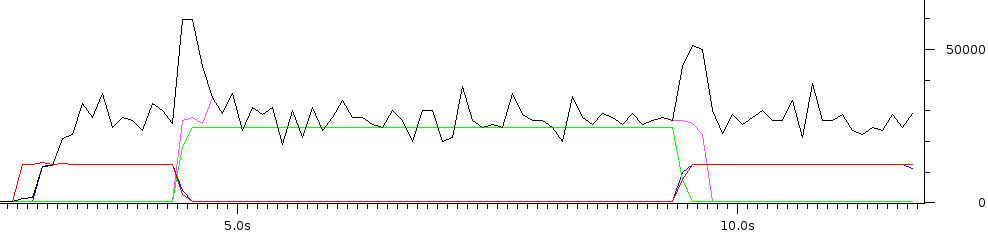
\includegraphics[width=\textwidth]{2trein3rau}
    \caption{Pakketstromen tussen de centrale en de RAU's in het RoF-model.  De horizontale as is de tijdsas, verticaal staat de doorstroom in \textit{Bytes per tick}.  E�n tick is 0,1~s waardoor de waarde 50.000 op de grafiek overeenkomt met 500.000~Bps of 4~Mbps.  De rode lijn geeft de hoeveelheid verkeer weer naar RAU0, terwijl de groene en blauwe dit doen voor RAU1 respectievelijk RAU2.  De paarse lijn geeft een indicatie van het verkeer afkomstig van RAU1, waar beide treinen zich op een bepaald moment samen bij bevinden.  De grootte van de totale stroom naar de centrale wordt weergegeven door de zwarte lijn.\label{RoF-2t3rau-centrale}}
  \end{center}
\end{figure}



\section{Evaluatie}
\npar Met deze resultaten hebben we aangetoond dat het moving cell concept een werkbare benadering kan zijn.  Het grote voordeel ten opzichte van de klassieke manier is dat de connectie nergens verloren gaat, de datastroom wordt nergens onderbroken.  Aan een dergelijke bewegingssnelheid is een connectie met traditionele WiFi-oplossingen helemaal onmogelijk, maar dit kan via het hier voorgestelde model verholpen worden.
\chapter{Conclusie}
\section{Besluit}
In deze masterproef wordt aangetoond dat het mogelijk is om een gebaar met een beperkt aantal voorbeelden bij te leren aan een convolutioneel neuraal netwerk, met behulp van het dieptebeeld van de Microsoft Kinect en GPU-acceleratie.
\npar In alle experimenten is te zien dat een groter aantal voorbeelden een positieve invloed heeft op de sensitiviteit of recall van de herkenning van het bijgeleerde gebaar. De stijging in deze waarde is het sterkst tussen het gebruik van 1 tot 10 samples. Voor het ideaal van one-shot learning ligt deze waarde voor 10 van de 20 gebaren boven de 10\%. Wanneer er 10 samples gebruikt worden zijn er 11 gebaren die meer dan 50\% sensitiviteit tonen. Het gebruikte model is relatief eenvoudig gehouden om meer experimenten te kunnen uitvoeren maar behaalt toch behoorlijke resultaten op deze uitdagende taak.
\npar Zowel precision als recall van het bijleren van een gebaar liggen in lijn met de prestaties van het basismodel waarin alle gebaren uit de trainset samen worden aangeleerd met alle voorbeelden. 
\npar Door het bijleren van twee nieuwe gebaren na elkaar wordt aangetoond dat het model dynamisch uitbreidbaar is. De sensitiviteit op de twee nieuw bijgeleerde gebaren van het experiment ligt zelfs hoger dan wanneer ze elk afzonderlijk worden bijgeleerd.
\npar De kloof tussen het herkenningsvermogen na bijleren met een beperkt aantal voorbeelden en het meteen aanleren van alle gebaren is wel nog steeds groot.
\section{Verder onderzoek}

Er is een eerste aanleiding gegeven tot one-shot learning en het dynamisch uitbreiden van het lexicon van een gebarenherkenningssysteem. Er is veel ruimte voor verbetering en verder onderzoek.

\npar Ten eerste is er weinig voorverwerking gedaan op de gebruikte data. Een extra voorverwerkingsstap kan bijvoorbeeld de achtergrond filteren en betere ruisonderdrukking voorzien. Zo zullen er betere en meer algemene features worden aangeleerd en gedetecteerd. Er kan ook gebruik gemaakt worden van alle frames van het beeld en driedimensionale convoluties om rekening te houden met het tijdsaspect.

\npar Het kan interessant zijn om een meer complex en state-of-the-art netwerk op te stellen en te trainen met een grotere dataset zoals de ``Chalearn Isolated Gesture Recognition (ICPR '16)'' dataset uit \cite{wan_chalearn_2016}. Deze bevat 48000 voorbeelden, bijna vijf keer zo veel als de ChaLearn LAP 2014 dataset die hier gebruikt werd, en beslaat 249 verschillende gebaren. Doordat er zo veel verschillende gebaren in deze dataset zijn kunnen er nog meer algemene features ge\"etraheerd worden. Meer algemene features levert meer potenti\"eel voor het bijleren van een gebaar en de dynamische uitbreiding van het herkenbaar lexicon.
\npar Er kan enkel met deze nieuwe dataset gewerkt worden op een analoge manier als in deze masterproef of er kan gekozen worden om gebaren bij te leren uit een andere dataset, zoals bijvoorbeeld de LAP 2014 dataset.
\npar Vanuit intu\"itie moet data-augmentatie veel helpen bij het bijleren vanuit weinig voorbeelden. Een doordachte data-augmentatie techniek die translaties, rotaties, vervorming en ruis toevoegt kan gunstige resultaten brengen op voorwaarde dat het model dat hiervoor wordt gebruikt genoeg parameters heeft om de grotere variatie te beschrijven.

\appendix


% De grafie en de index
\bibliography{bibliodatabase}

\backmatter
\listoffigures
%\listoftables
%\addcontentsline{toc}{chapter}{Lijst van codefragmenten}
%\lstlistoflistings

% lege pagina (!!)

% kaft



\end{document}
